\documentclass[a4paper, twoside]{IEEEtran}
\IEEEoverridecommandlockouts

% Dokumentation IEEEtran LaTeX class
% https://ras.papercept.net/conferences/support/files/IEEEtran_HOWTO.pdf

\usepackage{csquotes}
\usepackage[english]{babel}
\usepackage[noadjust]{cite}
\usepackage{amsmath,amssymb,amsfonts}
\usepackage{algorithmic}
\usepackage{graphicx}
\usepackage{textcomp}
\usepackage{xcolor}
\usepackage{balance}
\usepackage{float}
\usepackage[all]{nowidow}
\usepackage{listings}
\usepackage[hidelinks]{hyperref}
\usepackage{url}
\usepackage[capitalise]{cleveref}
\usepackage{booktabs}

\lstdefinestyle{python}{
    language=Python,
    escapechar=!,
    captionpos=b,
    basicstyle=\small\ttfamily,
    keywordstyle=\color{blue},
    stringstyle=\color{red},
    commentstyle=\color{gray},
    breaklines=true
}

% don't judge
\hbadness=10000

% group citations
\renewcommand{\citepunct}{,\penalty\citepunctpenalty\,}
\renewcommand{\citedash}{--}

\begin{document}

\title{Project Report—CoDes: Co-Design of Serverless Platforms and Applications}

\author{
    \IEEEauthorblockN{
        Valentin Carl\IEEEauthorrefmark{1},
        Daniel Gottschling\IEEEauthorrefmark{2},
        Jonas Heisterberg\IEEEauthorrefmark{2},
        David Schmidt\IEEEauthorrefmark{2}, and
        Marvin Steinke\IEEEauthorrefmark{1}
    }\\
    \IEEEauthorblockA{
        Technische Universität Berlin\\
        Email:
        \IEEEauthorrefmark{1}\{carl, marvin.steinke\}@tu-berlin.de,
        \IEEEauthorrefmark{2}\{d.gottschling, heisterberg, d.schmidt\}@campus.tu-berlin.de
    }
}

\maketitle
\thispagestyle{plain}
\pagestyle{plain}

\begin{abstract}
    Wow, what an abstract!
\end{abstract}

\setcounter{tocdepth}{1}
\tableofcontents

\section{Introduction}\label{sec:introduction}

\section{Nuclio}
\label{sec:nuclio}

%%%%
\subsection{A Customizable Serverless Platform}
\label{sec:nuclio-introduction}
To better understand the following subsections and the language they contain, we begin with a basic overview of Nuclio as our framework. Nuclio is an open-source serverless platform designed for data-intensive, compute-intensive workloads. Unlike widely known cloud-based solutions such as AWS Lambda\footnote{\url{https://aws.amazon.com/de/lambda/}} or Google Cloud Functions\footnote{\url{https://cloud.google.com/functions}}, Nuclio offers the flexibility to deploy serverless functions directly on your own infrastructure on an open source basis. This allows for greater control and customisation and opens up possibilities that might be limited on vendor-bound platforms.
The open source nature of Nuclio allows us to optimize the platform based on specific project requirements and to experiment flexibly with new concepts to improve performance and cost metrics. This adaptability led our project manager, Trevor Schirmer, to select Nuclio for our work and further developments.

\subsection{Architecture components}
\label{sec:nuclio-components}
Nuclio's architecture includes several key components: Trigger, Processor, Worker, Controller, Builder, Dashboard and Scaler. Triggers, activated by event sources, initiate actions that are handled by processors. They can be divided into the following event classes\footnote{\url{https://nuclio.io/latest/concepts/architecture/}}:
\begin{itemize}
    \item Synchronous request/response - the client makes a request and waits for an immediate response, e.g. HTTP
    \item Asynchronous message queue request - messages are distributed to the subscribers, e.g. RabbitMQ\footnote{\url{https://www.rabbitmq.com/}}
    \item Message or record streams - an ordered set of messages or record updates are handled sequentially, e.g.  Kafka\footnote{\url{https://kafka.apache.org/}}
    \item Record or Data Polling - a filtered set of data objects is retrieved from an external data source or database, e.g.  DynamoDB\footnote{\url{https://aws.amazon.com/de/dynamodb/}}
\end{itemize} 
This project report is limited to the HTTP-based request-reply trigger, which was already used intensively in previous work by Schirmer et al. \cite{schirmer2023profaastinate}.
A processor listens for one or more of the triggers and executes user functions with one or more parallel workers\footnote{\url{https://nuclio.io/latest/introduction/}}. 
The workers use language-specific runtimes to execute the function; a distinction is made between the types:
\begin{itemize}
    \item Native - real-time routines based on Golang or C.
    \item SHMEM - the processor communicates with the SHMEM function runtime via zero-copy shared memory channels, e.g. Python
    \item Shell - for command line execution functions or executable binary files\footnote{\url{https://nuclio.io/latest/concepts/architecture/}}.
\end{itemize}
\vspace{5mm} 
\begin{figure}
    \centering
    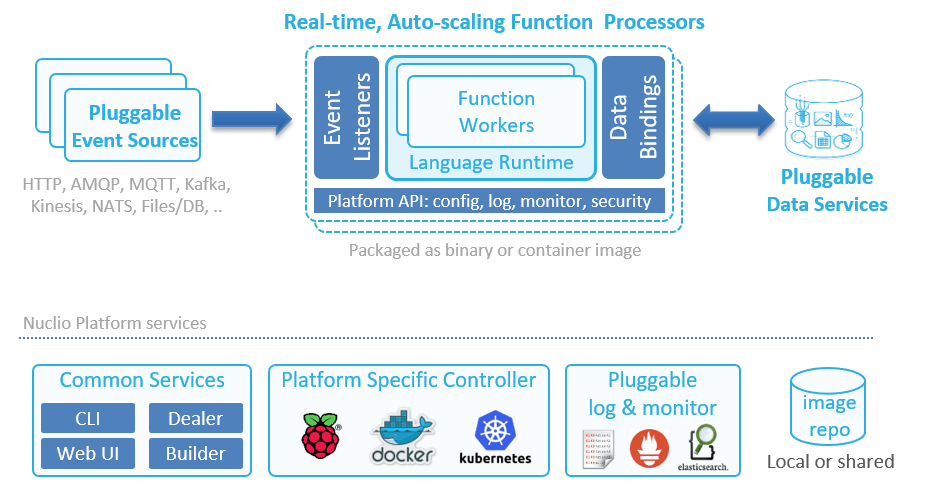
\includegraphics[width=0.48\textwidth]{figures/profaastinate/nuclio-architecture.png} % Adjust the width as needed
    \caption{
         Nuclio's high-level architecture\protect\footnote{\url{https://nuclio.io/latest/introduction/}}.
    }
    \label{fig:nuclio-architecture}
\end{figure}

The dashboard is a standalone microservice that is accessed via HTTP and contains a code editor GUI. The user can access this or alternatively the nuclio CLI to provide function code via the function registry. However, in order to be able to execute the function in the worker, the builder is required, which builds a binary file or a container image from raw code and optional build instructions and dependencies, which is pushed to an image repository\footnote{\url{https://nuclio.io/latest/introduction/}}.

In this work, the dashboard was mainly used to write the function code, working only with a local registry, primarily using a Native and SHMEN worker for Go and Python. 

\begin{figure}
    \centering
    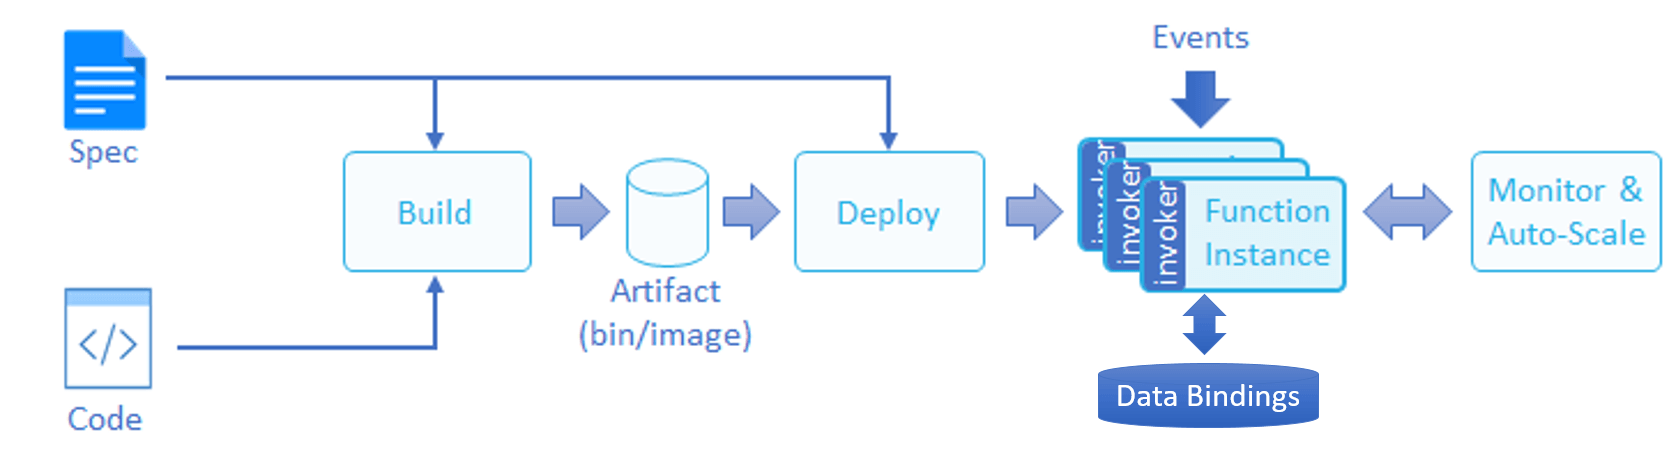
\includegraphics[width=0.48\textwidth]{figures/profaastinate/nuclio-build-deploy.png} 
    \caption{
         Function build and deployment flow\protect\footnote{\url{https://nuclio.io/latest/concepts/architecture/}}.
    }
    \label{fig:nuclio-build-deploy}
\end{figure}

A controller then connects the various components by receiving the specifications of functions and event sources. It invokes builders and processors via an orchestration platform and manages function elasticity, lifecycle and versions.

\label{sec:nuclio-namespace}
All the resources, such as functions or triggers, that are described earlier, can then be logically grouped or isolated in a Nuclio Namespace. This enables better control of user access and authorization. 

The Nuclio system as a whole can then be run in different environments, either as standalone Docker containers or on container orchestration tools like Kubernetes. Our research focused mainly on the Docker and Minikube container environments. The latter is a local cluster\footnote{\url{https://minikube.sigs.k8s.io/}} of the orchestration platform Kubernetes\footnote{\url{https://kubernetes.io/}}. 

Finally, it is worth noting that certain Nuclio features, such as "scale to zero", are exclusively accessible in on-premises environment of Iguazio's Nuclio Enterprise Edition, facilitating efficient function execution\footnote{\url{https://www.iguazio.com/}}.
% - intro: motivation fusionize, presentation of implementation of paper
%   concept with a real faas platfrom, nuclio
%   - use figs 2 and 3 from paper

\section{Fusionize}\label{sec:fusionize}

%this section goes into more detail of the briefly introduced Fusionize paper
%it presents the implementation strategy of this paper and explains all
%components
%ti presents a guide of how a user setups their Fusionizer-enabled tasks

This section further examines the \textsc{Fusionize} paper that was briefly
introduced earlier. It details the implementation strategy for the paper's
concepts and clarifies its various components. Additionally, a user guide is
provided to assist the process of setting up their Fusionizer-enabled tasks.

\subsection{Concept}

\textsc{Fusionize}, by Schirmer et al. \cite{schirmer2023fusionize} is a
feedback-driven framework that automates the setup of composite task-based
applications on cloud FaaS platforms. As outlined in Figure
\ref{fig:fusionize_highlvl}, it takes unchanged FaaS tasks and enhances their
performance and cost-efficiency by iteratively modifying their deployment
configuration and inlining tasks based on monitored performance.

\begin{figure}
    \centering
    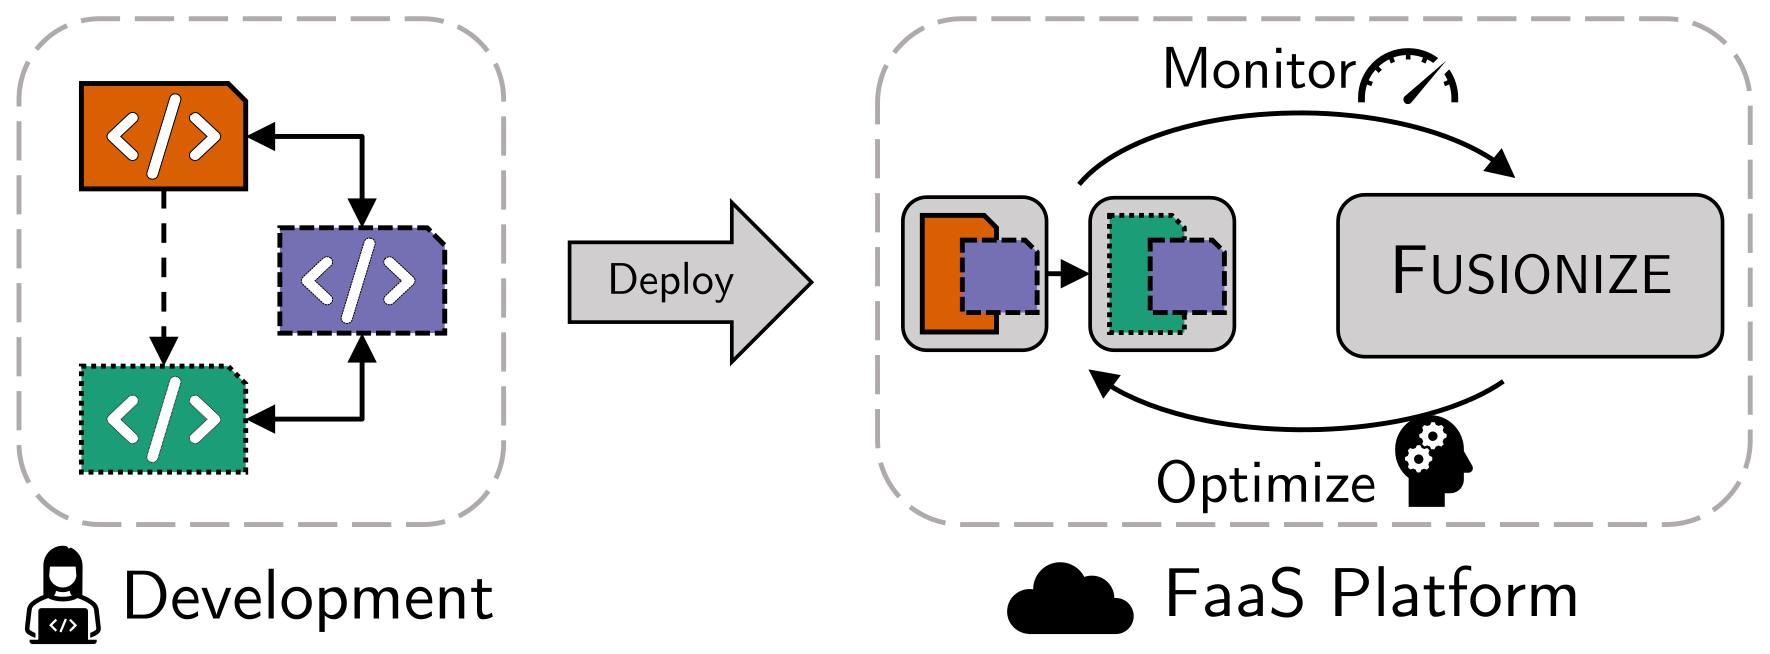
\includegraphics[width=\linewidth]{figures/fusionize_highlvl}
    \caption{
        High-level overview of \textsc{Fusionize} \cite{schirmer2023fusionize}.
        \textsc{Fusionize} optimizes FaaS tasks' performance and cost by
        altering deployment configurations and inlining tasks within FaaS
        functions.
    }
    \label{fig:fusionize_highlvl}
\end{figure}

The concept of inlining from compiler theory is used to expand remote FaaS
function calls with task source code where beneficial, a concept known as
function fusion. Function fusion can reduce remote call overheads and confine
cold start cascades.

Using the familiar FaaS programming model, \textsc{Fusionize} processes current
FaaS applications and infers their call patterns, cost efficiency, and
performance from live execution behavior. It then continuously optimizes the
application setup for cost efficiency and end-to-end performance. If application
behavior changes, \textsc{Fusionize} can automatically adapt to this new
environment and optimize further.

In the context of \textsc{Fusionize}, \emph{task} refers to any software
function that developers construct, while \emph{function} denotes an executable
deployment artifact. Each function contains a single \emph{fusion group}, which
is a set of tasks executed as part of the function.

\subsection{Implementation Overview}

The initial concept for implementation with Nuclio was to develop a new function
processor that would manage the inlining of functions. These would be selectable
during the function deployment phase. However, the underlying platform component
of Nuclio and its Kubernetes (k8s) implementation does not account for the
possibility of mapping multiple tasks to a single function. A consultation with
the Nuclio developers revealed that a complete rewriting of the platform would
be required to enable this functionality. This proved unrealistic within the
scope of this project for a single developer.

Instead, an independent \emph{Fusionizer} server, developed in Python, is
introduced between the user and a non-modified, \emph{vanilla} Nuclio platform.
As depicted in Figure \ref{fig:fusionizer_highlvl}, the user only interacts with
the Fusionizer server, not Nuclio directly. The server provides a REST API for
task management, adopting the same function configuration for tasks as with
deployment via Nuclio.

\begin{figure}
    \centering
    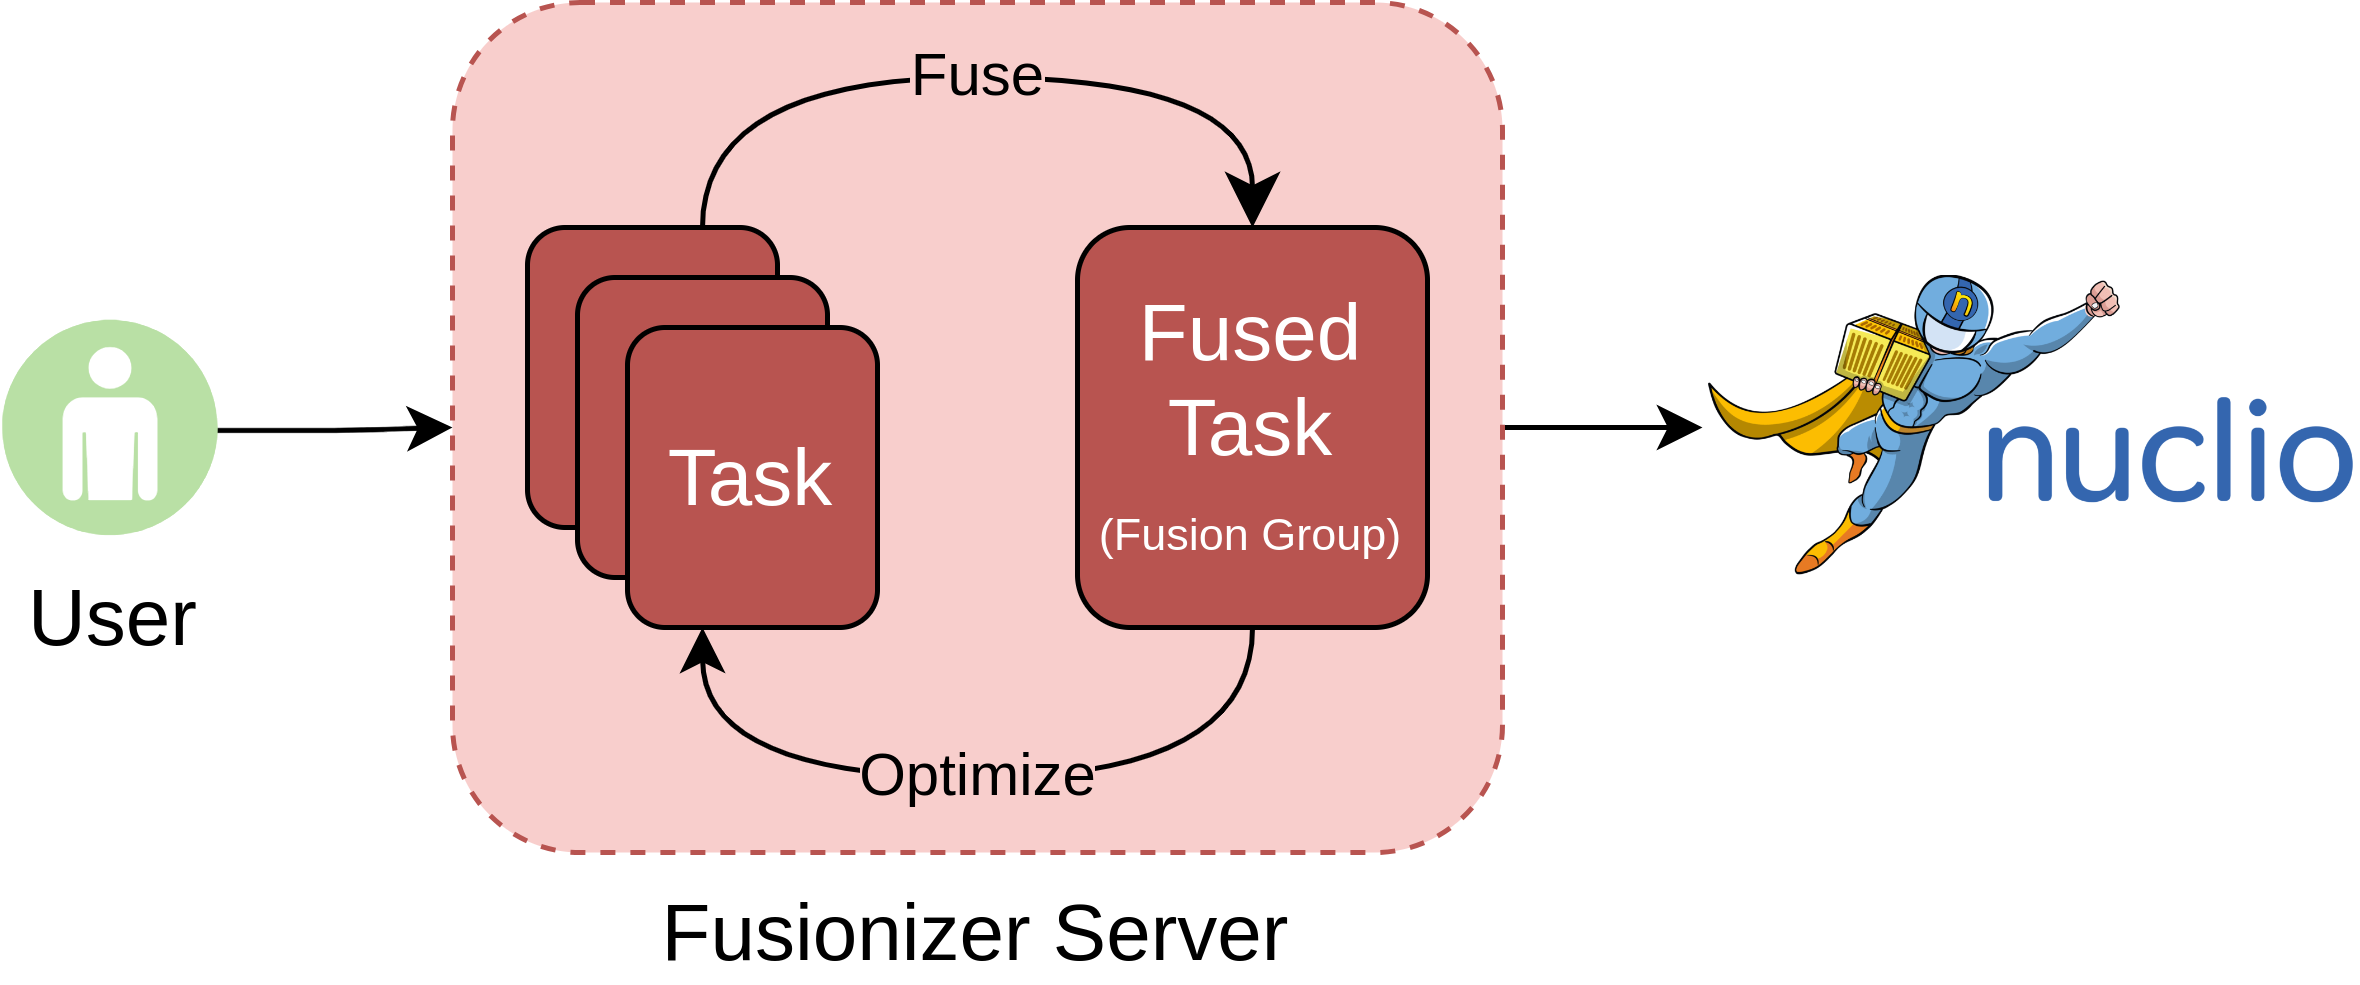
\includegraphics[width=\linewidth]{figures/fusionizer_highlvl}
    \caption{
        High-level implementation overview. The user does not deploy or invoke
        their tasks through nuclio, but the Fusionizer server which applies the
        concepts of \textsc{Fusionize}.
    }
    \label{fig:fusionizer_highlvl}
\end{figure}

Users deploy their fine-grained application code to the Fusionizer server. The
server then groups tasks into fusion groups, according to an optimization
strategy. Each of these groups are fused into a single Nuclio function and
deployed to the platform. Each Nuclio function deployed from the Fusionizer
server contains a dispatcher component. This component routes invocation
requests from the Fusionizer server to the appropriate task. Additionally, HTTP
invocation requests between two tasks contained within the same Nuclio function,
or fusion group, are intercepted and invoked locally. To minimize network
overhead, the Fusionizer server is housed on the same machine as Nuclio. This
implementation, however, only enables the concepts presented in the paper and
does not represent any optimization strategies.

This strategy offers significant advantages as it can be executed without the
time-consuming task of comprehending and altering the existing codebase of
Nuclio. The applicability of this strategy is also not confined to Nuclio as the
single FaaS platform, as further detailed in Section X.

\subsection{Components}

This section reviews the individual components that compose the Fusionizer
server and provides a more detailed view. The overall relationship between these
components is visually represented in Figure \ref{fig:fusionizer_components}.
The main components involved in this system are the API server, the nuctl
interface, the Optimizers, the Task Fuser, and the Dispatcher.

\begin{figure}
    \centering
    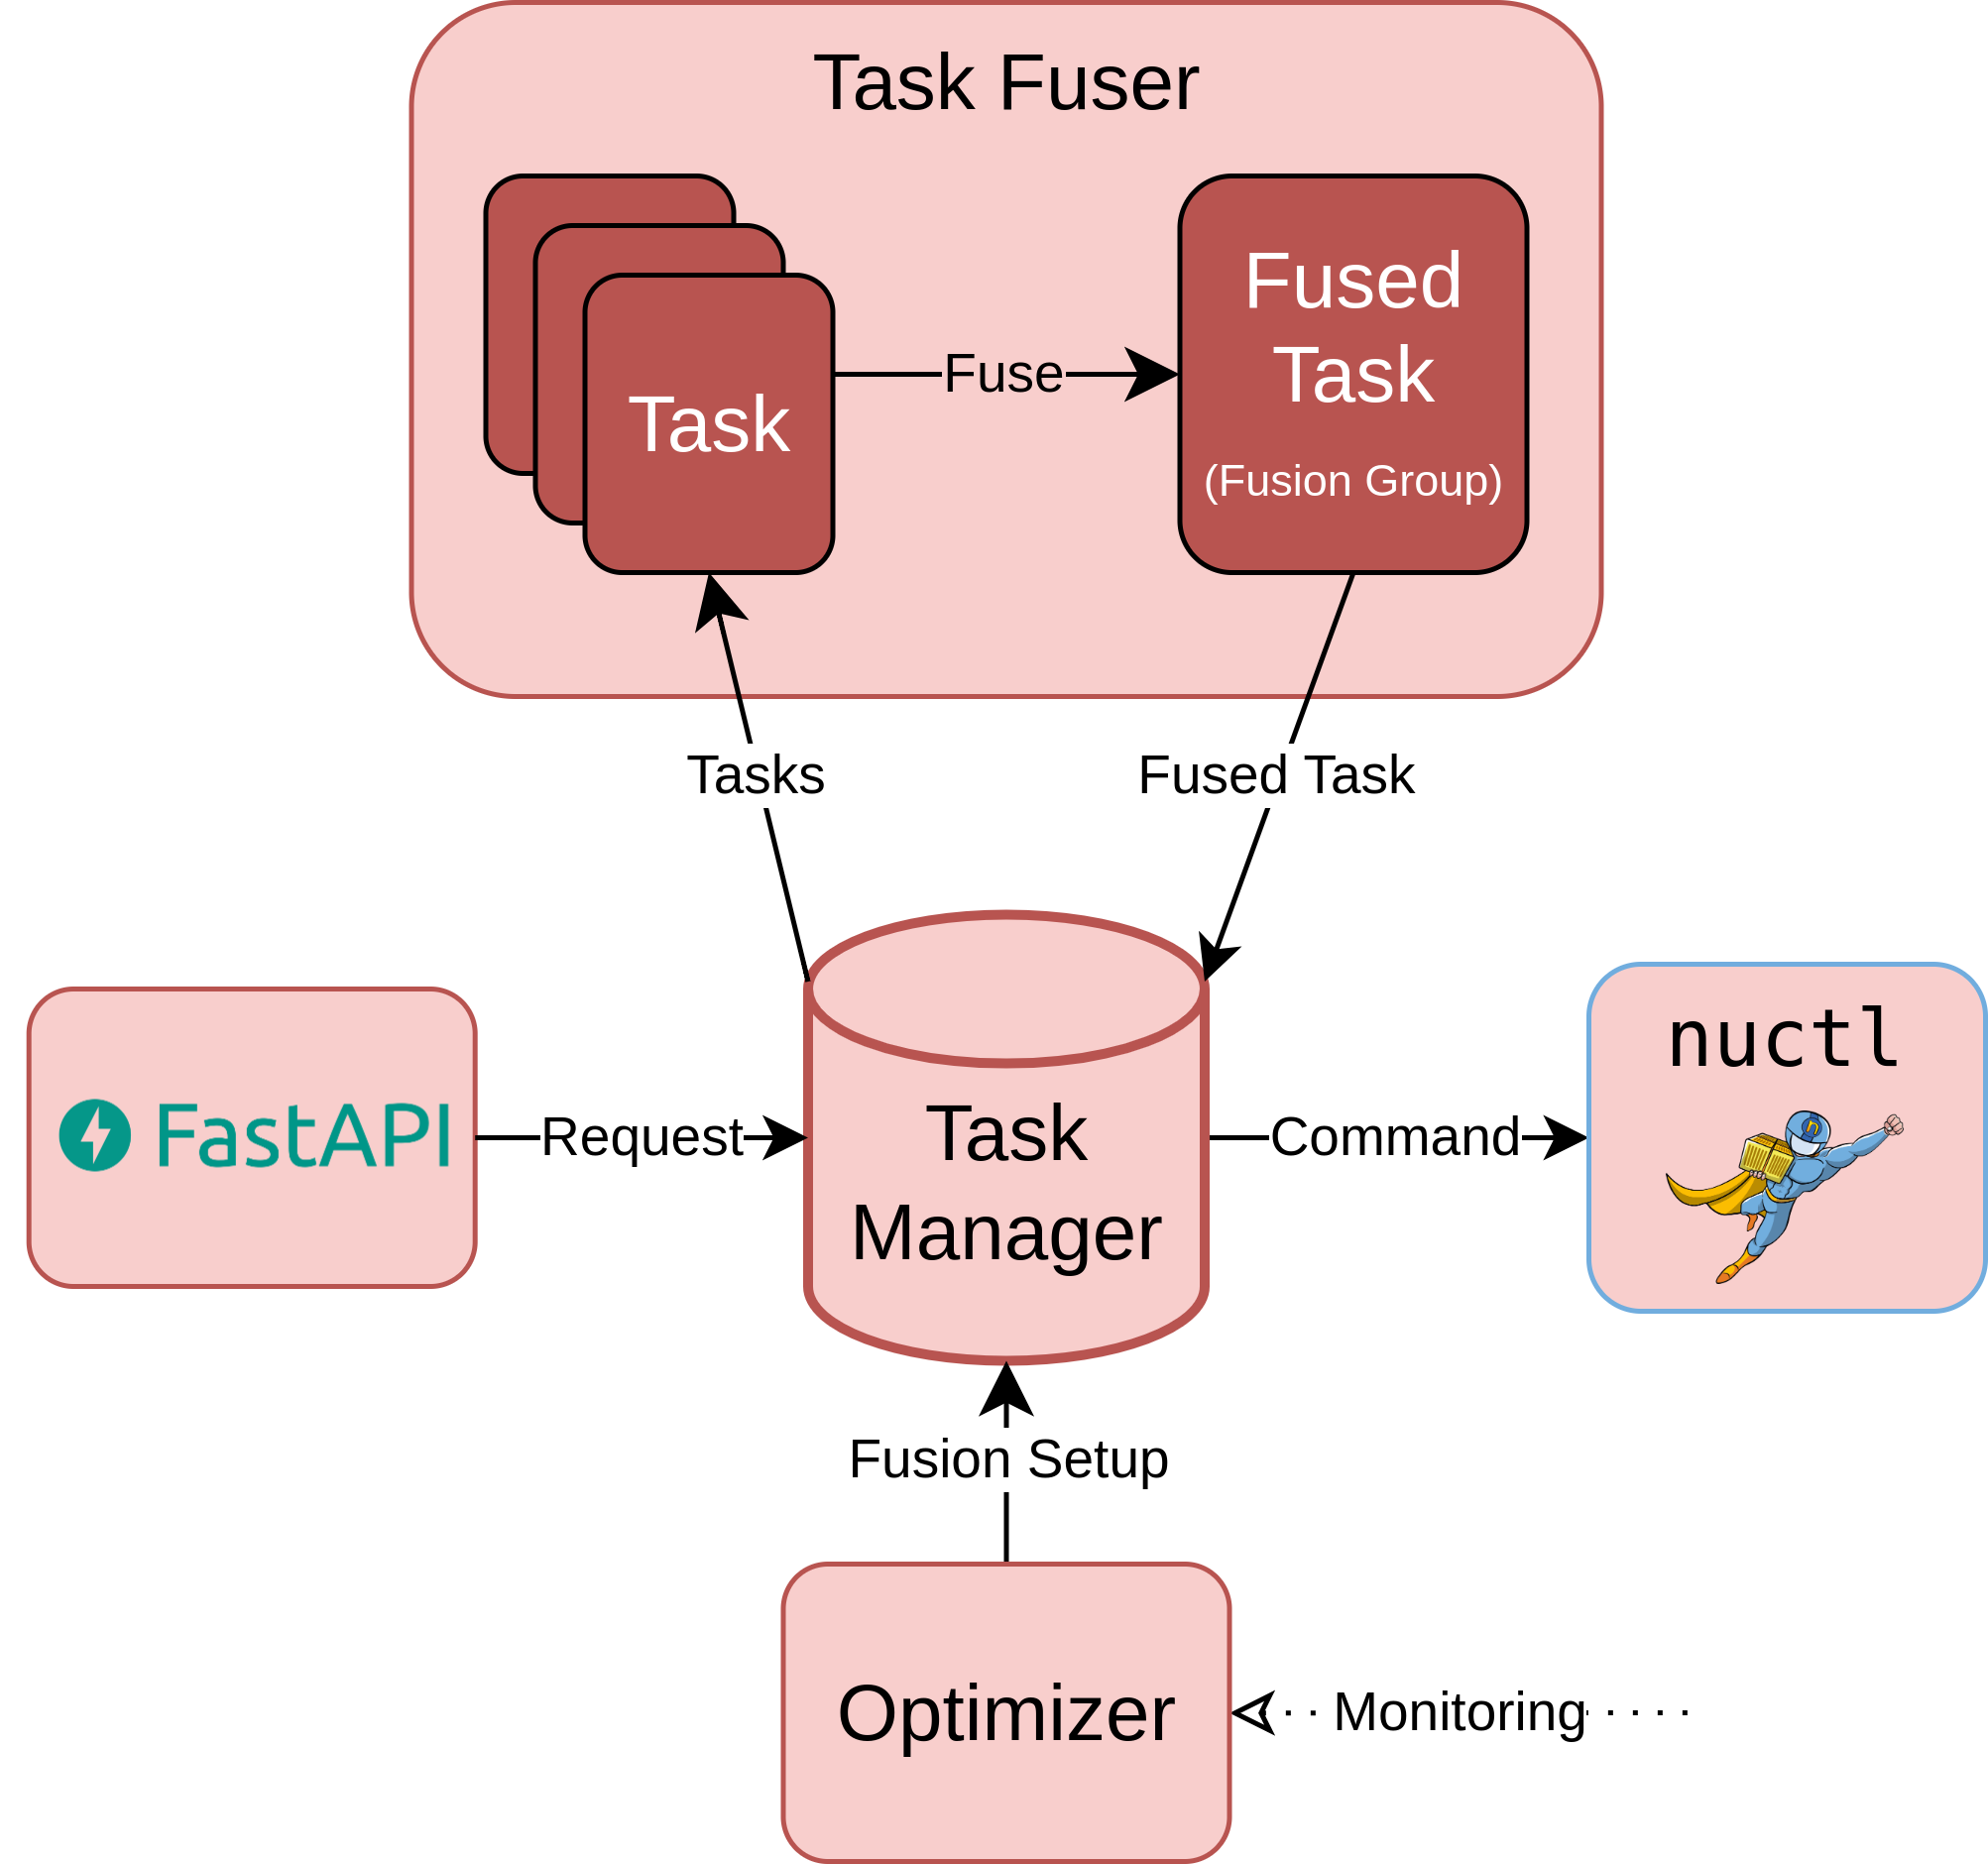
\includegraphics[width=.8\linewidth]{figures/fusionizer_components}
    \caption{
        Fusionizer server components. The API server forwards incoming requests
        to the Task Manager. Then, following the fusion setup configured by the
        Optimizer, tasks are dispatched to the Task Fuser. Here, tasks are
        merged into a Nuclio function which is subsequently deployed through the
        nuctl interface.
    }
    \label{fig:fusionizer_components}
\end{figure}

\subsubsection{API Server}

%api server offers RESTful api to the user this FastAPI based server provides
%HTTP interface for user interaction with the fusionizer system. api can be seen
%in Table 1 the http endpoint always stays the same and is structured like
%http://<url>/<task-name>/

The API server provides a RESTful API to the user, acting as a FastAPI-based
server. It offers an HTTP interface which facilitates seamless user interaction
with the Fusionizer system. Information regarding the API can be found detailed
in Table \ref{tab:fusionizer_api}. The structure of the HTTP endpoint remains
consistent and takes the form of \url{http://server-address:8000/task-name/}.

\begin{table}
    \centering
    \caption{Fusionizer HTTP API}
    \label{tab:fusionizer_api}
    \resizebox{\linewidth}{!}{
        \renewcommand{\arraystretch}{1.4}
        \begin{tabular}{|c|c|c|c|}
            \hline
            \textbf{Action} & \textbf{Method} & \textbf{Headers} & \textbf{Body} \\
            \hline
            Invoke Task & POST & Content-Type: application/json & \textit{args} \\
            \hline
            Deploy Task & PUT & Content-Type: multipart/form-data & \textit{zip file} \\
            \hline
            Delete Task & DELETE & - & - \\
            \hline
            Get Task Info & GET & - & - \\
            \hline
        \end{tabular}
    }
\end{table}

\subsubsection{nuctl Interface}

%this component is a wrapper for Nuclio's command-line interface (CLI), which
%provides command-line access to Nuclio features. directly translates API from
%Table 1 to nuctl commands except for taks invocations task invocations are
%handled via Nuclio's HTTP API. For this, the specific address for each Nuclio
%function is retrieved via the nuctl "get" command where the
%"internalInvocationUrl" is used as the endpoint for function calls

This component serves as a wrapper for the command-line interface (CLI) of
Nuclio\footnote{nuctl.
\url{https://nuclio.io/docs/latest/reference/nuctl/nuctl/}}, providing
command-line accessibility to various Nuclio features. It enables the direct
translation of the API from Table \ref{tab:fusionizer_api} into nuctl commands,
excluding task invocations. Task invocations are specifically managed through
the use of Nuclio's HTTP API. The unique address for each Nuclio function is
obtained through the \texttt{nuctl get} command, in which the internal
invocation url is employed as the endpoint for the function calls.

\subsubsection{Task Manager}

The Task Manager is responsible for overseeing the organization and lifecycle
management of tasks within fusion groups. It has the capacity to allow for the
dynamic reconfiguration of fusion groups, a process based on external
configurations from an Optimizer. Its functions extend to deploying new tasks
and fusion groups, as well as updating the existing groups with new setups and
eliminating outdated groups. This includes overseeing deployments to Nuclio.

In terms of updating the fusion setup, the Task Manager plays a vital role in
authenticating changes and managing the deployment of either revised or new
fusion groups, and the deletion of old groups, which ensures consistent task
operation. This involves determining which fusion groups remain the same, which
are new and need deployment, and which are deemed outdated and thus require
deletion. It then proceeds to deploy new or altered fusion groups and discard
the obsolete ones. This process involves an attempt to fuse and deploy new
groups, using the Task Fuser and the nuctl interface, while also enabling the
deletion of old groups

If a specific task needs to be removed from the fusion setup and it is part of a
fusion group, that group will need to undergo modifications or, in some
scenarios, will have to be deleted entirely. In the instance of group
modification, the group's name is regenerated based on the remaining tasks.
Build directory information might also have to be edited or cleared entirely to
reflect these changes. The revised group is then primed for re-deployment,
excluding the removed task. If the group does still contain tasks post removal,
it is then re-fused and re-deployed, while the original group containing the
deleted task is eliminated from the setup.

\subsubsection{Optimizers}

%Optimizers provide way to easily implement custom optimization strategies each
%Optimizer needs to subclass the Optimizer abstract base class and implement: -
%the strategy: every optimization cycle, Optimizers apply an optimization
%strategy - sleep time: between these cycles, a halting duration must be
%specified after each cycle, the new fusion setup is sent to the Task Manager,
%either as JSON or as a list of fusion group objects example: Static Optimizer
%implements a static optimization strategy for Fusion Group configurations,
%based on predefined setups read from a JSON file this file contains
%predetermined Fusion Group configurations mapped to specific timestamps,
%indicating when to change configurations. it uses the current timestamp to
%decide when to pause execution and for how long, based on the timestamps
%defined in the configuration file. It initially sleeps until the time for the
%first configuration change is reached. it optimizes the Fusion Setups by
%selecting the configuration corresponding to the current timestamp from the
%JSON configuration file If there are no further configurations to switch to (no
%next timestamp is found), the Static Optimizer stops its execution.

Optimizers offer a convenient method for executing custom optimization
strategies. Any optimizer must be a subclass of the Optimizer abstract base
class, and it is expected to implement an optimization strategy which is brought
into play for every optimization cycle. Furthermore, a specific sleep time
should be implemented for the duration between these cycles. At the end of each
cycle, the new fusion setup is submitted to the Task Manager. This can be done
either in the form of a JSON or as a list of fusion group objects.

An example of an optimizer is the Static Optimizer. This implements a static
optimization strategy for fusion group configurations, the setups for which are
predefined and read from a JSON file. Each file contains pre-set fusion group
configurations that correspond to particular timestamps, which signals when to
transition between configurations. The current timestamp is used to decide when
to halt execution and for what duration, as specified in the timestamps within
the configuration file. Initially, the execution sleeps until the time assigned
to the first configuration change is reached. The Static Optimizer then
optimizes fusion setups by selecting the configuration linked to the current
timestamp from the JSON configuration file. If there no further configurations
present to switch to (if there is no subsequent timestamp identified), the
Static Optimizer concludes its execution.

In a practical context, defining the best fusion setup might necessitate the
consideration of factors such as resource usage and task load distribution. In
such instances, it is beneficial to implement an optimization strategy that
includes monitoring metrics.

\subsubsection{Task Fuser}

%The Task Fuser in its current form only handles Python tasks developed according
%to Nuclio's Python reference. This requires a task to have a handler script and
%a function configuration YAML file.
%
%The Task Fuser sets up a build directory for each fusion group that is to be
%deployed. it copies each task's files into it Then Merges multiple YAML
%configuration files into a single file. important for combining the
%configurations of multiple tasks into a single deployment, ensuring all the
%necessary settings and dependencies are consolidated.
%
%Task Fuser copies the Dispatcher library to the fusion group’s build directory.
%This script will later be used to dispatch requests to the appropriate task
%based on the configuration.
%
%Finally, Task Fuser generates a Python script that serves as the entry point for
%the fused deployment which supplies the Dispatcher with all tasks' handler
%scripts.

The Task Fuser currently operates solely on Python tasks that are built based on
Nuclio's Python reference\footnote{Nuclio Python Reference.
\url{https://nuclio.io/docs/latest/reference/runtimes/python/python-reference/}}.
This requires that a task includes both a handler script and a YAML function
configuration file. For each deployment, the Task Fuser prepares a designated
build directory for each fusion group. It duplicates each task's files into this
directory. In addition, it merges multiple YAML configuration files into a
singular file.

The Task Fuser then copies the Dispatcher library into the build directory of
the fusion group. This script is later utilized to appropriately dispatch
requests to the correct task, as per the configuration. Finally, a Python script
is generated by the Task Fuser that acts as the entry point for the fused
deployment, providing the Dispatcher with handler scripts from all tasks.

\subsubsection{Dispatcher}

%as depicted in Figure 4, the Fusionizer Dispatcher is deployed with a fusion
%group to form a Nuclio function
%the Dispatcher routes incoming requests to the correct task
%from the outside, or from Nuclio's point of view, there is only function.
%so, to target a specific task for invocation, an HTTP header is used by the
%Fusionizer server to tell the dispatcher, which task to route the request to
%The Dispatcher also handles traffic between tasks in the same function (or
%fusion group) which is the most important functionality of the whole project as
%this avoids routing the request over network which causes remote call overheads
%and cold start cascades.
%for this the Dispatcher utilizes a custom http adapter from the requests
%library. This adapter is given to all tasks' handlers which they must use to
%make http requests.
%the adapter checks if the requested address is the Fusionizer server and if the
%requested task is located in the current local fusion group. If so, the task is
%invoked locally, else the request is handled like a regular HTTP request.

\begin{figure}
    \centering
    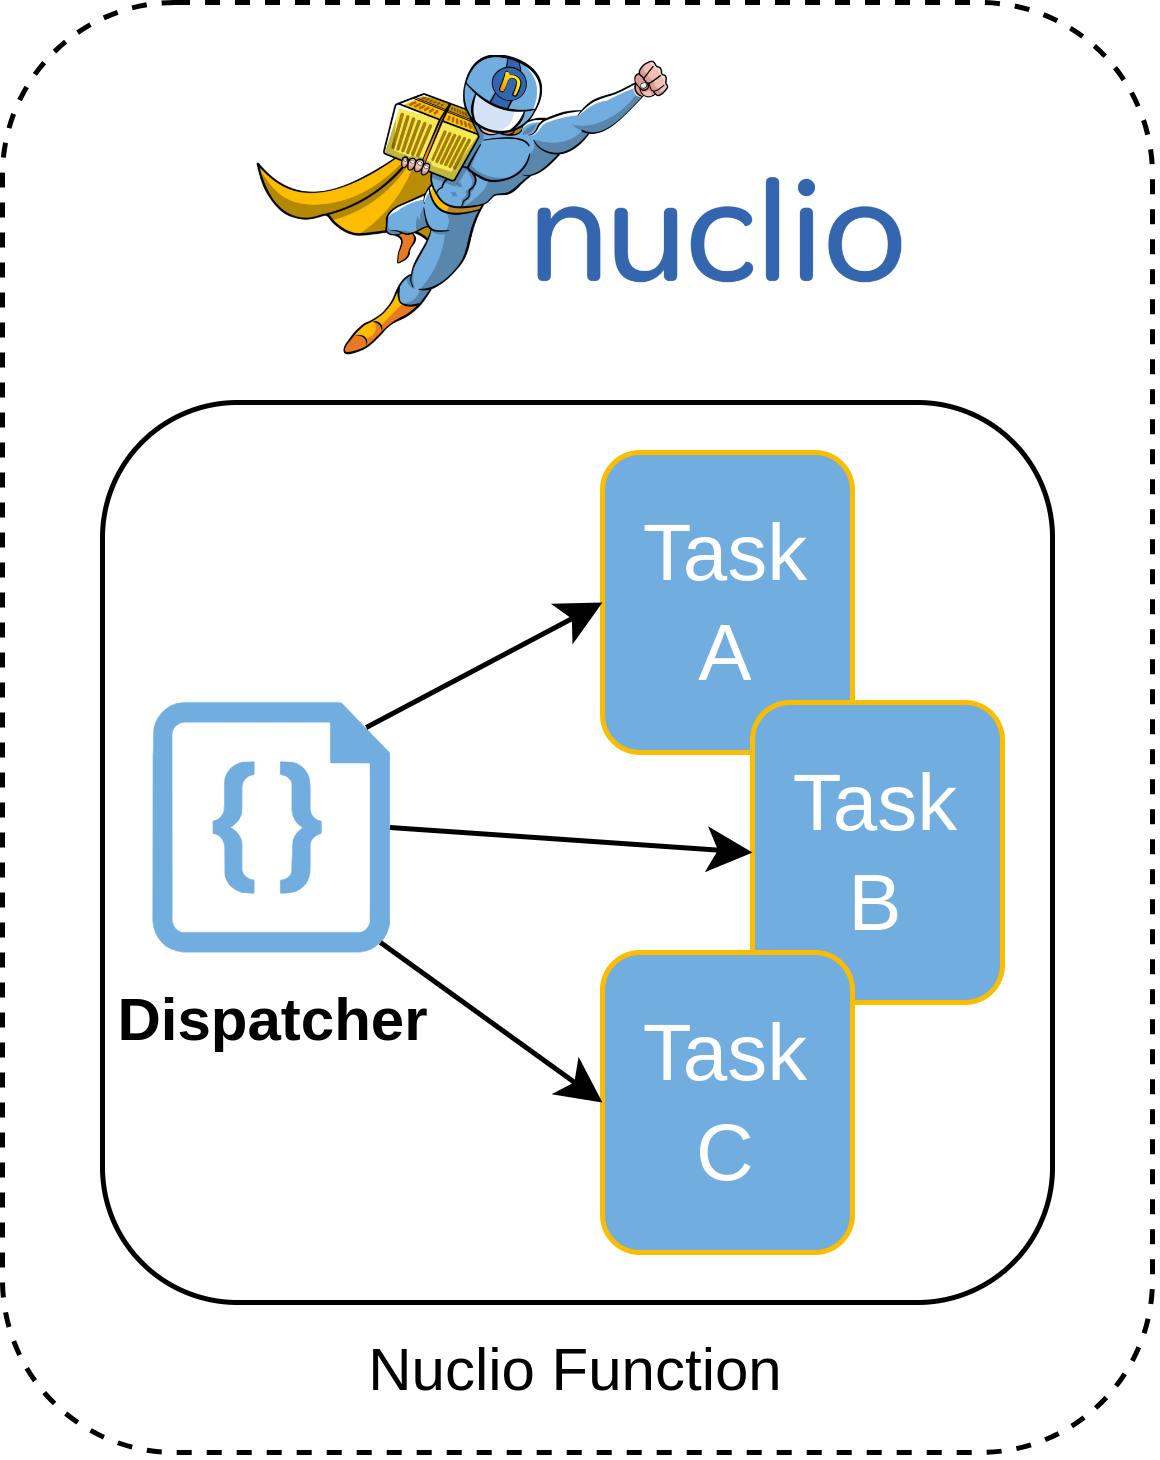
\includegraphics[width=.5\linewidth]{figures/fusionizer_dispatcher}
    \caption{
        The Fusionizer Dispatcher routes incoming requests to the correct task
        within a Nuclio function, manages intra-group traffic, and can locally
        invoke a task if it resides within the local fusion group.
    }
    \label{fig:fusionizer_dispatcher}
\end{figure}

Figure \ref{fig:fusionizer_dispatcher} illustrates the integration of the
Fusionizer Dispatcher with a fusion group to establish a Nuclio function. The
primary role of the Dispatcher is to direct incoming requests to the appropriate
tasks. From the perspective of the exterior or from Nuclio, this appears as a
single function.

In order to pinpoint a specific task for invocation, the Fusionizer server
utilizes an HTTP header to communicate to the Dispatcher which task should
receive the request. The Dispatcher holds a secondary role of managing traffic
between tasks within the same function, or fusion group, which is crucial due to
its ability to bypass the need for routing requests across the network. This
eliminates the issues of remote call overheads and cold start cascades.

The Dispatcher achieves this through the use of a custom HTTP adapter, obtained
from the requests library. This adapter is provided to the handlers of all
tasks, which is then employed to make HTTP requests. The adapter verifies
whether the requested address is related to the Fusionizer server, and if the
target task is located within the current local fusion group. If both conditions
are met, the task request is invoked locally. Otherwise, the request proceeds as
a standard HTTP request.

\subsection{User Function Setup}

%users have to provide a handler script and a configuration YAML file
%the handler script is like previously mentioned based on Nuclio's Python
%reference. The only difference is that Fusionizer enabled Python functions need
%to have an additional parameter in their handler method called
%requests_session. This is the custom HTTP adapter as detailed in the previous
%section. When making HTTP request, users are encouraged to use this session

Users are required to supply both a handler script and a configuration YAML
file. As previously noted, the handler script should be based on Nuclio's Python
reference. However, Fusionizer-enabled Python functions need to feature an
additional parameter in their handler method named \texttt{requests\_session}.
This serves as the custom HTTP adapter that enables local task invocation
interception, as detailed in the previous section. For making HTTP requests,
users are encouraged to utilize this session. The usage of this requests session
in a handler method is outlined in Listing \ref{lst:example_handler}.

\begin{figure}
    \begin{lstlisting}[
        style=python,
        caption={
            Example handler method that showcases the usage of the custom
            requests session that is needed, when invoking other
            Fusionizer-enabled tasks.
        },
        label={lst:example_handler}
    ]
def handler(context, event, !\textbf{requests\_session}!):
    fusionizer = event.headers[
        "Fusionizer-Server-Address"
    ]
    # invoke other Task
    task = "task42"
    url = f"http://{fusionizer}:8000/{task}"
    headers = {
        "Content-Type": "application/json"
    }
    data = {"value1": 5, "value2": 3}
    # use custom requests session
    response = !\textbf{requests\_session}!.post(
        url,
        headers=headers,
        json=data
    )
    return response.text
    \end{lstlisting}
\end{figure}

%setup of the YAML configuration file stays the same. Users only need to watch
%out for compatibility across tasks since the Nuclio function they are deployed
%with only has one configuration. Tasks are therefore e.g. incompatible when:
%- they have the same dependencies with different versions
%- have different min and max replica count
%- cpu limitations
% A tasks description is also omitted in favor for its fusion group's
% description

The setup of the YAML configuration file remains consistent. Users must simply
be mindful of task compatibility due to the fact that the Nuclio function within
which they are deployed only has a single configuration. Consequently, tasks can
become incompatible under certain conditions such as sharing the same
dependencies but with varying versions, having diverse minimum and maximum
replica counts, or possessing differing CPU limitations. A task's description is
also excluded, in favor for the description of its fusion group.

\subsection{k8s Deployment}

The core part of this deployment is the Pod \emph{nuclio-fusionizer}. This Pod
operates the Nuclio Fusionizer container, which is based on the supplied docker
image\footnote{Fusionizer Docker Image.
\url{ghcr.io/marvin-steinke/nuclio-fusionizer:latest}}. The container within the
Pod is configured to listen for incoming connections on port 8000. It is set up
with the service account \emph{nuctl-sa}, in order to enable interaction with
the k8s API. The deployment specifies volume mounts to the host Docker socket
and application configuration. Because the Nuclio Fusionizer utilizes Nuclio's
nuctl component, which in turn employs Docker, the utilization of the host's
Docker socket is favored over the less efficient Docker-in-Docker (DiD)
alternative. Permissions for the service account are provided through a Role and
RoleBinding. The Role \emph{nuctl-enabler} provides a range of permissions
across various API groups and resources. These resources include ingresses,
nuclio CRDs, services, configmaps, pods, secrets, and deployments, all of which
facilitate the operation of nuctl.

\section{SAND}\label{sec:sand}

In this section, we introduce the main ideas behind SAND, describe our implementation for Nuclio and the components in detail, and compare our implementation to that of Akkus et al.~\cite{akkus2018sand}.

\subsection{Concepts}

When building serverless applications, it is important to connect the invocations of different functions into function chains or workflows.
Because FaaS-platforms often host functions of different applications for different users, providing isolation between functions is a critical issue.
It should not be possible for a function to access the data of functions deployed by other users, for example.
At the same time, functions of the same application typically requires less isolation between each other than functions of different applications.
Akkus et al.~refer to this idea as \enquote{two-level fault isolation}~\cite{akkus2018sand}.
In turn, reducing isolation between functions (of the same application) can lead to performance improvements.
Instead of trying to optimize individual functions, we can reduce the total workflow duration by reducing the latency between steps of a workflow.
Similarly, allowing different functions to access shared data can improve the platform's resource usage. 

To demonstrate these ideas, Akkus et al.~present SAND~\cite{akkus2018sand}.
SAND is a serverless platform that aims at improving application performance by reducing the isolation between functions of the same application.
Figure~\ref{fig:sand_architecture} shows an overview of SAND's architecture.
The platform consists of the following components.
\begin{itemize}
    \item \emph{Grain}: A grain is an individual FaaS function.
    \item \emph{Application}: An application is a set of functions and the workflows defined for these functions. It can span across multiple hosts.
    \item \emph{Sandbox}: An application has its own container on a host, which is the sandbox. 
    \item \emph{Message bus}: A message bus is a means for functions of the same application to communicate. 
    \item \emph{Grain worker}: A grain worker is a function worker. It loads the function code and its dependencies, subscribes to the grain's queue, and invokes the function accordingly.
\end{itemize}

\subsubsection{Application Sandboxing}\label{subsub:application_sandboxing}

\begin{figure}
    \centering
    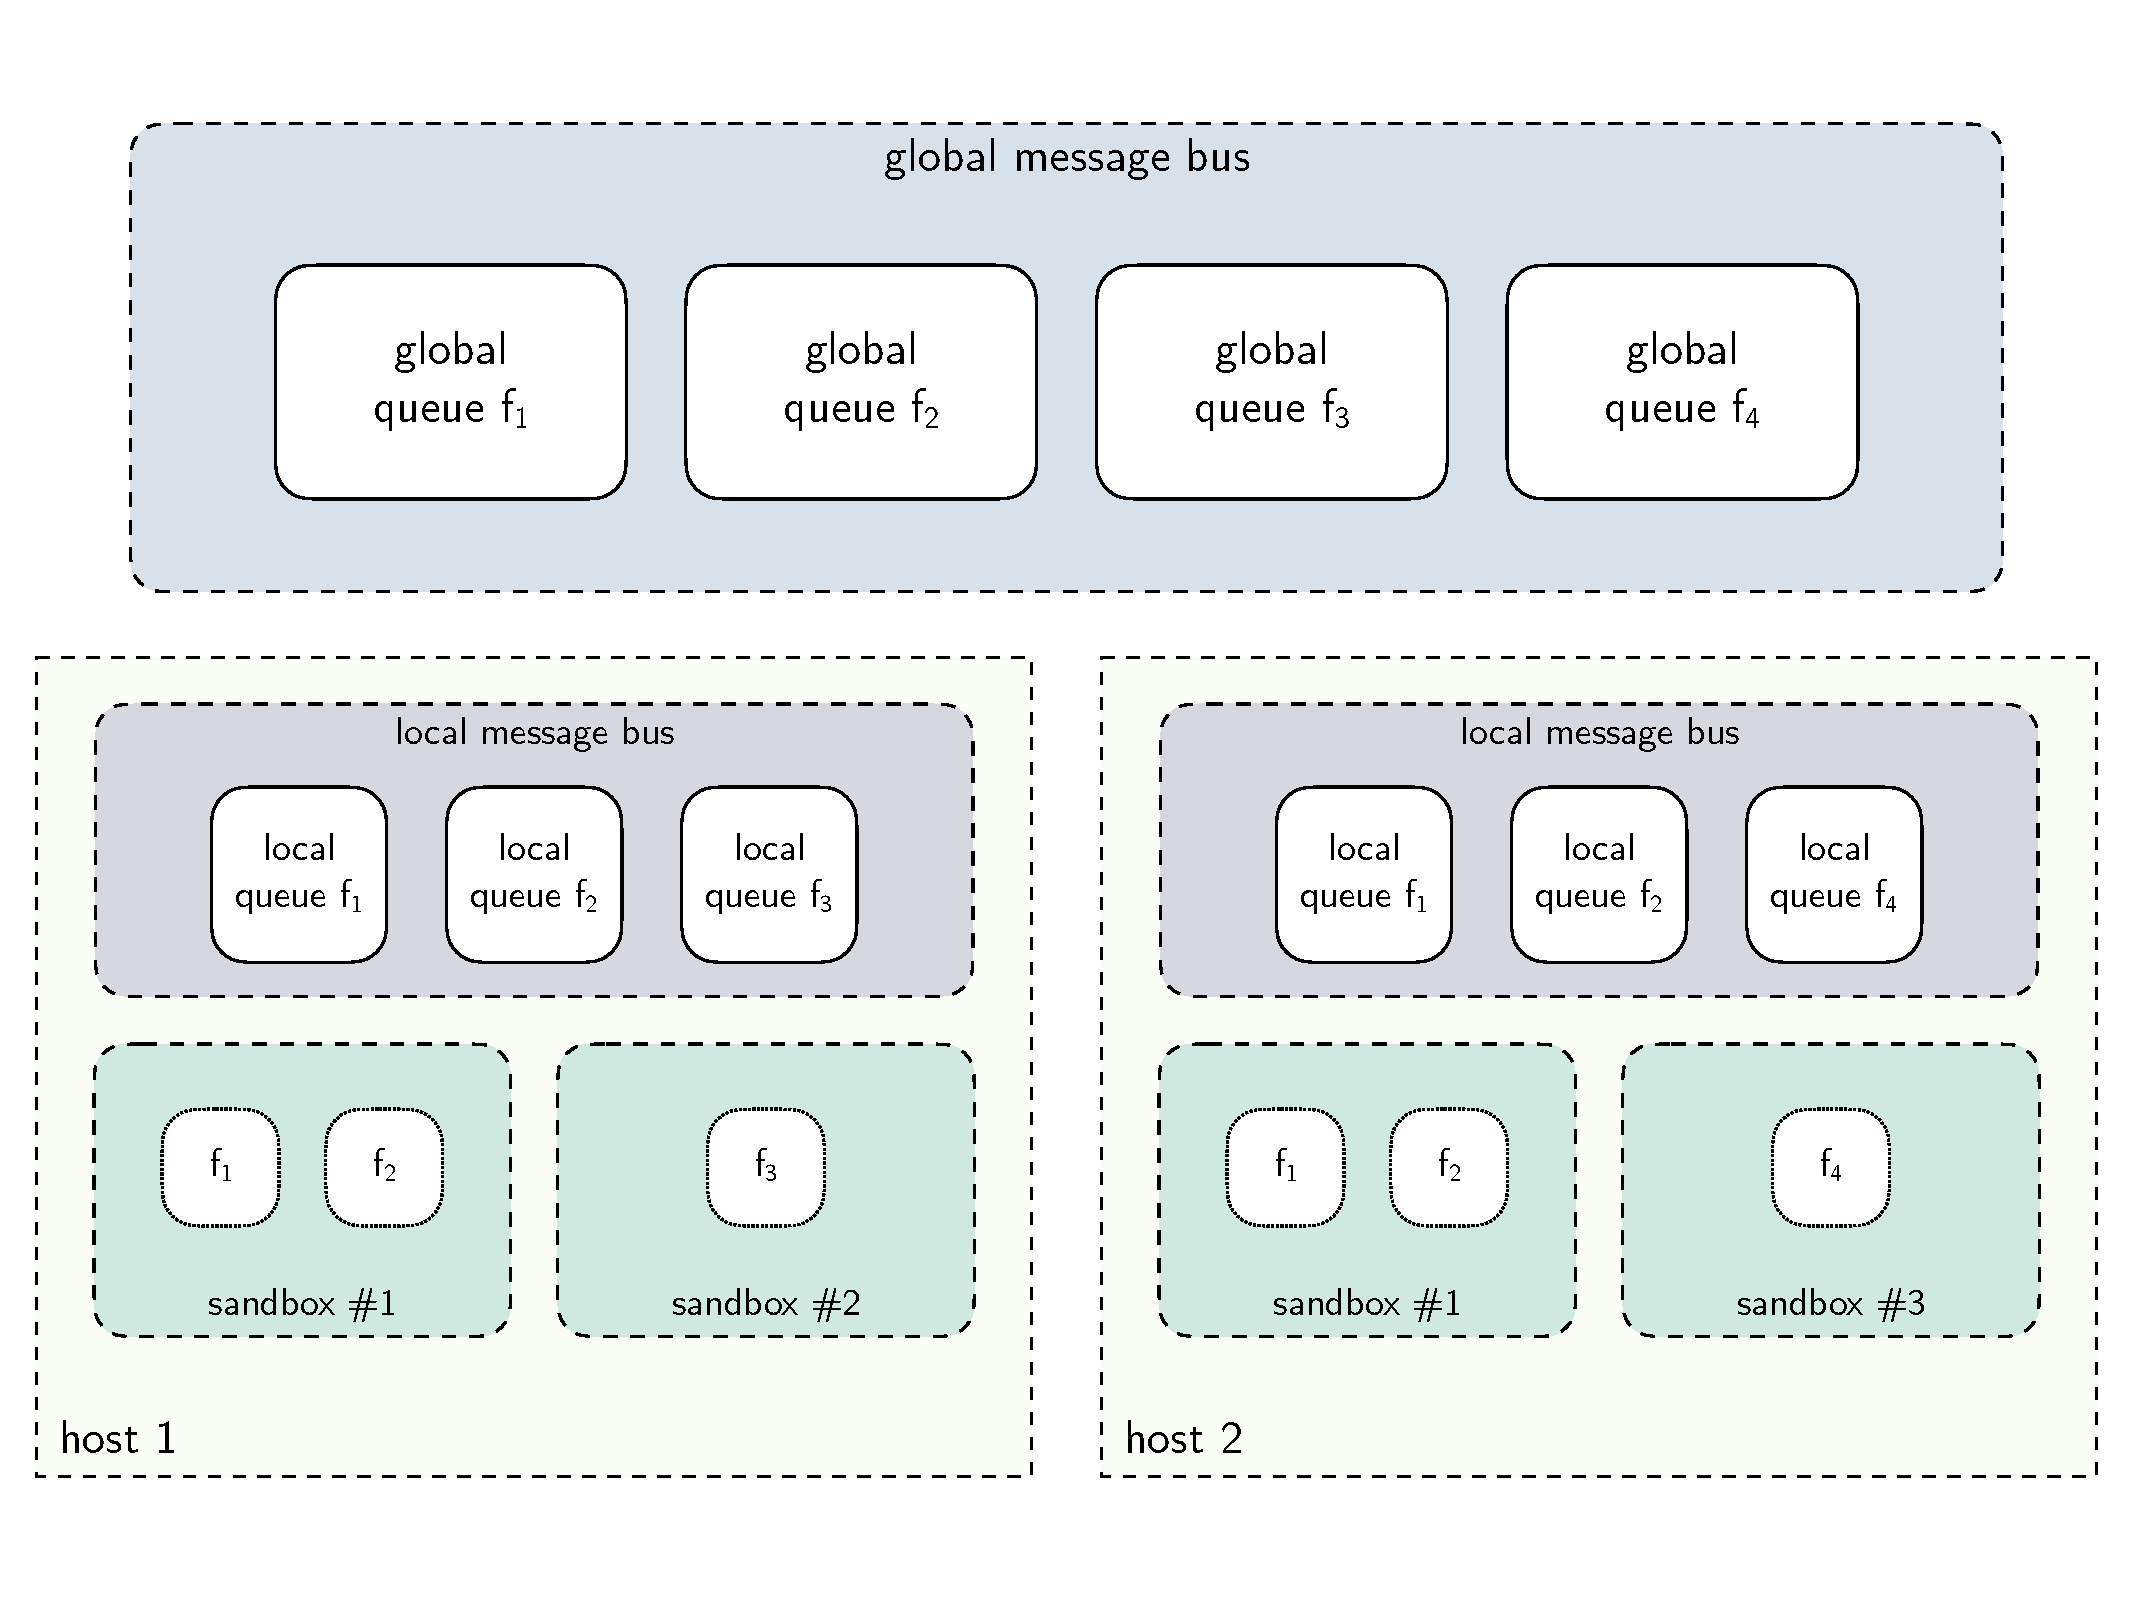
\includegraphics[width=\linewidth]{figures/sand_architecture.pdf}
    \caption{
        SAND's architecture comprises multiple hosts, multiple applications spanning across multiple hosts, sandboxes on the hosts containing different functions in addition to a local message bus, and a global message bus~\cite{akkus2018sand}.
    }\label{fig:sand_architecture}
\end{figure}

In order to realize these benefits while keeping isolation between functions of different applications, Akkus et al.~introduce \enquote{application sandboxing}~\cite{akkus2018sand}.
They list different technologies and options for implementing two-level fault isolation, among which are VMs, containers, unikernels, processes, and threads.

SAND uses Docker containers for their sandbox implementation~\cite{akkus2018sand}.
Each application runs in a different container, and the functions making up the applications run as different processes.
To handle incoming requests, SAND uses process forking.
The benefits of this approach are threefold.
\begin{itemize}
    \item The startup latency using process forking is far lower than the startup latency using new containers for function invocations.
    \item Libraries shared by functions only need to be loaded once in an application.
    \item Memory use increases only slightly with new function invocations, and the memory is released immediately once the function call is over, which leads to more efficient resource usage.
\end{itemize}

\subsubsection{Hierarchical Message Queuing}

To implement a workflow in a serverless platform that does not explicitly provide means of function chaining, functions typically invoke the workflow's next step by sending requests to the platform in the same way an external invocation would be sent.
This is inefficient from both the perspective of the platform and of the workflow developer.
For the platform, this creates additional load as internal requests compete for resources with external requests at the platform's gateway.
For the workflow developer, this adds potentially high latency between function calls, which increases the total workflow duration and end-to-end latency, in turn.

SAND can run in a distributed manner across multiple hosts.
In addition, it is possible for an application to span multiple hosts.
For example, the application could consist of more functions than a single SAND host can handle, or the application might be distributed across multiple regions with improved function placement.
Consequently, functions of the same application need to be able to communicate with other functions running on the same and on different hosts.

As SAND treats internal and external requests differently, it provides two additional options for functions to communicate.
This allows SAND to have \enquote{shortcuts for functions that interact with each other}~\cite{akkus2018sand}.
\begin{itemize}
    \item The \emph{local message bus} allows functions in the same sandbox to communicate.
    \item The \emph{global message bus} handles invocations across hosts and serves as backup for the local message buses.
\end{itemize}
Here, a message bus is a set of FIFO queues, containing one queue per function, where each messages in a queue corresponds to a function call.

\subsection{Implementation Overview}

Akkus et al.~implemented SAND using Docker containers for application sandboxing~\cite{akkus2018sand}.
To implement a similar feature for Nuclio, we need to adapt their design to fit better for Nuclio's design.
Nuclio offers two backends for deploying functions: Docker and Kubernetes, where the Docker backend is intended for development purposes and the K8s backend for production. 
Therefore, the SAND implementation for Nuclio should reflect the focus on Kubernetes.

While using the Kubernetes backend, Nuclio deploys a new pod for each function, which contains only one container for the function processor, respectively.
Using the same abstraction level as SAND—as in using containers for application sandboxing—does not reflect Nuclio's use of Kubernetes well, and it seems infeasible given the scope of Nuclio's codebase. 
Taking this into account, we choose Kubernetes pods as our means of application sandboxing.

% TODO maybe remove the arrows
\begin{figure}
    \centering
    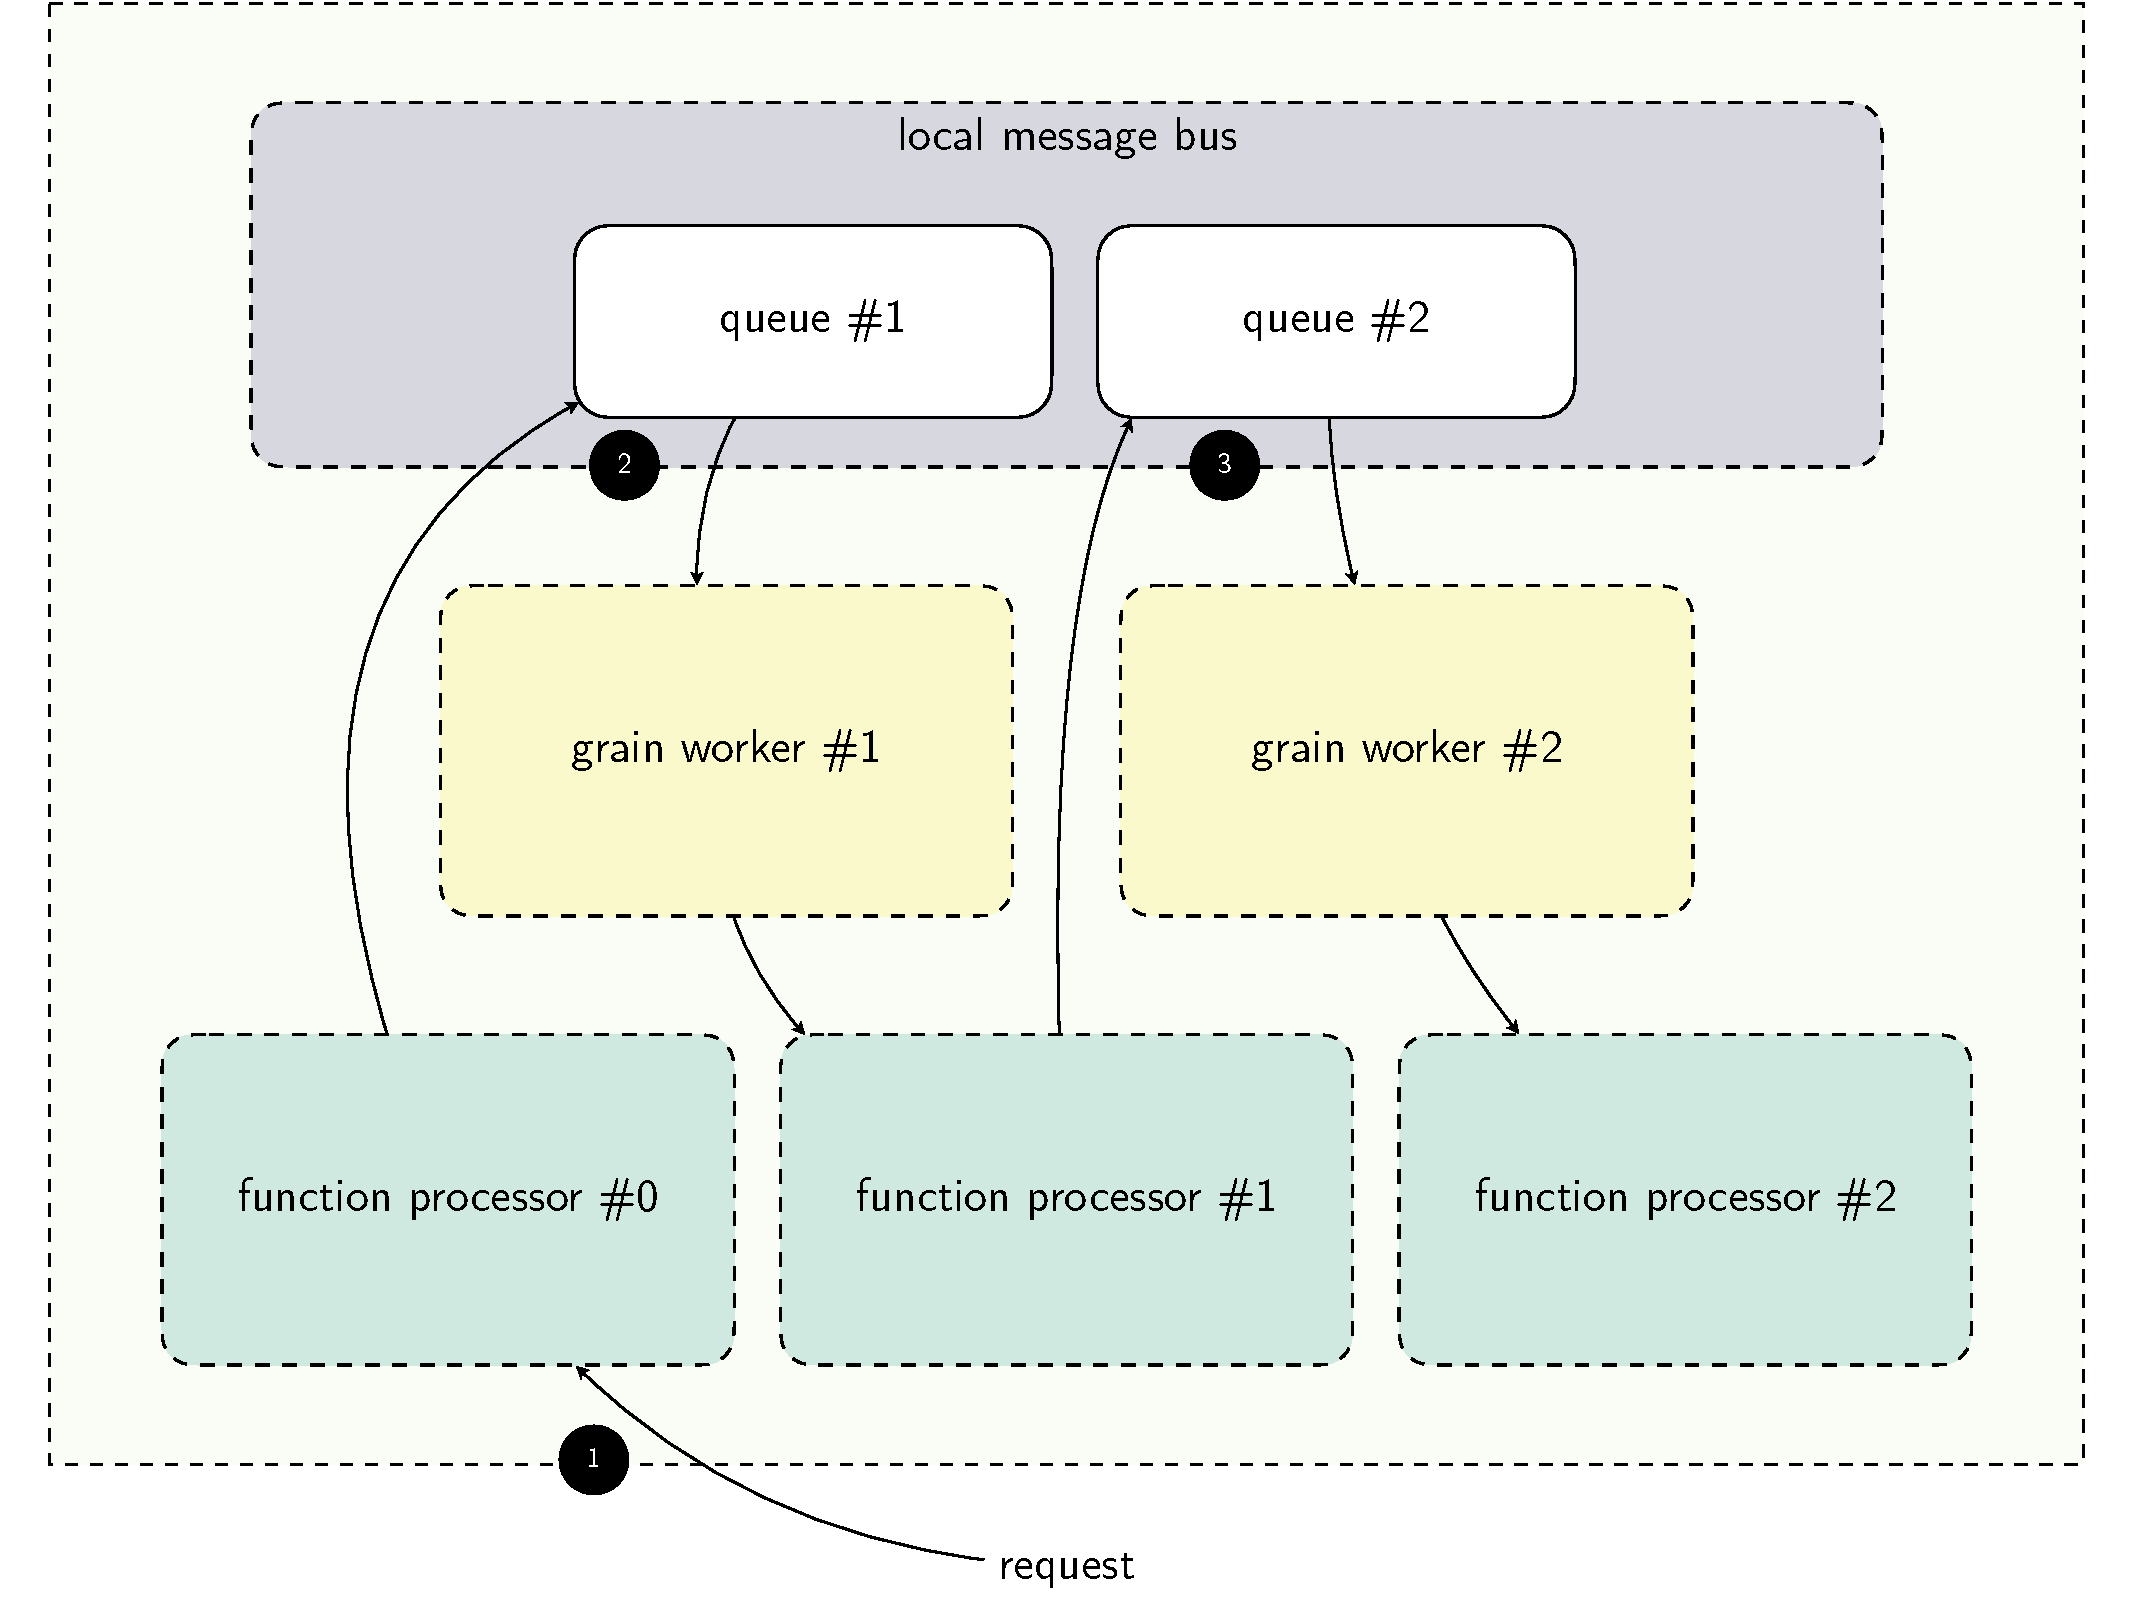
\includegraphics[width=\linewidth]{figures/sandbox.pdf}
    \caption{
        Our implementation of application sandboxing in Nuclio uses Kubernetes pods for isolation and contains containers for function processors, grain workers, and a local message bus. 
        Workflow steps are invoked by sending messages to the local message bus, which the next grain worker receives and uses to invoke its function.
    }\label{fig:sandbox}
\end{figure}

This way, our implementation merges Nuclio's function pods to create application sandboxes. Figure~\ref{fig:sandbox} shows an overview of our sandbox design, which contains $n$ containers for different function processors, $n-1$ containers for the grain workers, and a single container for the local message bus.

To invoke other functions, a function sends an AMQP message to the local message bus (which it can reach at \texttt{localhost:5672}). 
The queues have the same name as the functions for which they process requests, and the messages contain the function inputs. 
This allows the actual workflows to be determined dynamically at runtime depending on the functions' logic and their inputs.

Figure~\ref{fig:sandbox} also shows the general workflow process in the sandbox. 
\begin{enumerate}
    \item First, the Nuclio dashboard forwards an (external) request to the sandbox, where it is received directly by the workflow's first function. 
        The function is invoked, after which it invokes the next step by sending a message to queue corresponding to the workflow's next step.
    \item Next, the second function's grain worker—which is subscribed to \texttt{queue \#1}—receives the message and invokes its function.
        Again, the function is invoked, and it sends a message \texttt{queue \#2} after it has finished.
    \item Last, the second grain worker receives the message for the last step.
        It invokes its function, which concludes the workflow.
\end{enumerate}

When using the K8s backend, Nuclio can be distributed across multiple nodes, similarly to how SAND uses multiple hosts.
For implementing workflows across hosts, the Nuclio dashboard can be used as the global message bus. 
When calling functions of the same application in a different sandbox, the request is sent to the dashboard, which forwards it to the correct function.

\subsection{Components}

Next, we go over the different components of our implementation in more detail and highlight some differences to SAND.

\subsubsection{Sandbox}\label{subsub:sandbox}

In our implementation, a sandbox corresponds to a Kubernetes pod. 
Consequently, an application is a set of pods that run on different nodes, where the functions communicate through their local message bus or the Nuclio dashboard, depending on the location of the next function.

When deploying a function to its K8s backend, Nuclio creates a new \texttt{deployment} (which is a Kubernetes resource).
We modify this deployment to create custom application sandboxes.

To create a sandbox, we first require Docker images for the Nuclio function processors, as well as for the grain workers and local message bus.
Images for the function processors can be created using the builder that is accessible through the dashboard. 
As part of using Nuclio's K8s backend, we create a Docker registry that is used to push and pull Docker images for deploying new functions.
The images for the function processor have to be pushed into this registry.
In addition, we build a docker image for the grain workers and an image for the local message bus, which also have to be pushed to the registry.

Next, we modify the deployment configuration created for the workflow's first step to include all other components of the sandbox.
It is important to note that we have to modify the \emph{deployment} instead of, for example, the pod configuration. 
Otherwise, K8s will not add any additional containers to the previously created pod.
To add the additional containers to the pod, we list them under \texttt{spec.template.spec.containers} in the deployment configuration.
Here, we also set the ports and environment variables for the containers. 
The ports we set for the containers have to be unique; in K8s, \texttt{localhost} always refers to a pod.
Since containers in the same pod share their network space, networking between them becomes easier, but the ports used cannot overlap across containers.
For setting up the grain workers, we set the environment variables \texttt{FUNCTION\_NAME} and \texttt{FUNCTION\_PORT} to point to their respective function. 
It is also noteworthy that this approach to building sandboxes makes our SAND implementation compatible with our ProFaaStinate implementation.
To the Nuclio dashboard, it appears that the sandbox is a normal Nuclio function pod, and it starts the workflow as it would invoke any other function. 
Since our ProFaaStinate implementation modifies the Nuclio dashboard to allow asynchronous (and, consequently, the scheduling of) requests, the \emph{start} of the workflow can be delayed, too.

\subsubsection{Grain}

A grain is represented by a Nuclio function processor. 
For our use case, the grain carries the user's function, listens to HTTP requests, and invokes the function accordingly.
More general information on Nuclio's function processor can be found in
section~\ref{sec:nuclio}. % TODO TODO TODO

Nuclio's function processors contain workers to execute the user's code and different triggers to listen for requests.
We modified the HTTP trigger to be able to configure on which port it listens for HTTP requests inside the port using the environment variable \texttt{SAND\_PORT\_INTERNAL}.
Because of the intra-pod networking outlined above, function processors for different functions in the same pod cannot bind to the same ports, which made this change necessary.


\subsubsection{Grain Worker}

The grain workers are implemented as a Docker container running Alpine Linux 3.19\footnote{https://www.alpinelinux.org/} and Golang 1.21.4\footnote{https://go.dev/}.
When started, a grain worker looks for the environment variables set earlier (see~\ref{subsub:sandbox}) and subscribes to the respective queue at the local message bus.
If the queue does not yet exist, it is created by the grain worker.
For each message it receives from the local message bus, it sends an HTTP request to the correct function processor in order to invoke the function.

Within the sandbox, there exist $n$ grains and $n-1$ grain workers.
Since the workflow's first function is invoked directly by the request from the dashboard, there is no need for an additional grain worker for the first function.
Cyclic workflows could pose an exception to this; however, the sandbox' configuration can be easily adapted to fit this use case.

\subsubsection{Local Message Bus}

The local message bus is implemented a Docker container running Ubuntu 22.04 LTS\footnote{https://releases.ubuntu.com/jammy/}.
This container runs RabbitMQ, which we use as the message bus. 
We chose to use Ubuntu as the base image even though there is a RabbitMQ Docker image because the image is only community-maintained and less stable in our experience.
Conversely, using Ubuntu allows us to use the APT package \texttt{rabbitmq-server}, which is one of the recommended options\footnote{https://www.rabbitmq.com/docs/install-debian} for installing the message broker.

The container exposes the port 5672 to receive AMQP messages and 15672, which allows us to access RabbitMQ's management interface (with port forwarding). 

In the local message bus, there is one queue per function in the sandbox.
The queues are created automatically with the start of the grain workers. 
As part of AMQP, RabbitMQ has exchanges, where it received messages, and queues, to which the received messages are routed and from where it sends messages to any subscribed consumers.
For all messages, we use the default exchange.


\subsection{Differences to Akkus et al.'s Implementation}

Our implementation of application sandboxing and hierarchical message queuing differs in three ways from the implementation of Akkus et al.'s SAND~\cite{akkus2018sand}.
% 1 technologies
% 2 abstraction level for sandboxes
% 3 beginning of workflow process

\paragraph{Technologies}

Akkus et al.~\cite{akkus2018sand} use different technologies to implement their components. 
First, their prototype is implemented in Java and Python, while we use Golang as Nuclio is implemented in Golang.
Next, they use Apache Kafka for the global message bus and a custom Java-implementation for the local message bus, while we use RabbitMQ as Nuclio already offers a tech-preview for supporting RabbitMQ, which made it a good fit for the local message bus.\footnote{https://nuclio.io/homepage/rabbitmq/} 
In our implementation, we use the Nuclio dashboard as the global message bus.
In addition, SAND uses Apache Cassandra and NGINX.

\paragraph{Sandbox}

The next difference is in the level of abstraction for the implementation of application sandboxing.
In SAND, an application sandbox is implemented as a Docker container, while we use Kubernetes pods to this end. % TODO formulierung
Even though using containers leads to better performance by making communication between functions more direct, using pods instead fits better given Nuclio's use of Kubernetes.
Further, using containers for sandboxing would have required a near re-write of the function processors, which was infeasible with regard to the scope of the project. % TODO vielleicht lieber raus?

\paragraph{Workflow Process}

The last and smallest difference lies in the beginning of the workflow process. 
In SAND, after a request reaches the platform, the load balancer forwards it to the global message bus, where a grain worker handles it.
In contrast, requests go directly from the dashboard to the workflow's first function in our implementation.
The reason for this difference is that the Nuclio dashboard serves as load balancer and global message bus in our system.

\subsection{Limitations and Possible Improvements}

Our implementation has the following limitations.

\paragraph{Data Layer}

In addition to the hierarchical message queuing, the SAND platform also has a data layer, which allows the sharing of references to data instead of transferring the actual data between functions.
This data layer did not serve a large purpose in our project, as the implementation of application sandboxing and hierarchical message queuing in Nuclio was motivated by the comparison of total workflow durations of workflows between Fusionize and SAND.
However, adding this data layer does not pose a large challenge: In SAND, the (local) data layer is a key-value store \enquote{runs on each host similar to the local message bus}~\cite{akkus2018sand}.
In order to add this to our implementation, a key-value store can be added as an additional container inside an application's pod, which enables the same functionality. 

\paragraph{Pods as Sandboxes}

Using Kubernetes pods as sandboxes comes with a performance penalty, compared to other options listed in~\ref{subsub:application_sandboxing}.
This is to be expected, as Kubernetes pods are a significantly larger unit for sandboxing than, for example, using unikernels; however, it is still the best-fitting choice given Nuclio's design.

\paragraph{The Nuclio Dashboard}

Given that the Nuclio Dashboard treats the sandbox as a single function, we are not able to access other functions in the application with external requests. 
This is negligible for many use cases, where the start of the workflow is fixed, but this is still improvable.

\paragraph{Possible Improvement: Grain Workers}

A possible improvement is the direct integration of the grain workers into the function processors. 
The grain workers and the function processors' triggers serve a similar purpose: listen to events and invoke the function accordingly.
Currently, Nuclio offers a tech-preview for RabbitMQ triggers, indicating that improved support for the message broker can be expected in the future.
Once this is rolled out, the function processor could be configured to listen to the local message bus directly, which would make communication more direct and likely improve total workflow duration. 
However, this is only possible once Nuclio offers better support for RabbitMQ (or another event trigger), as is it not stable enough, yet.


\section{ProFaaStinate}
\label{sec:profaastinate}
% Das hier kann dann weg richtig?

The next section provides an overview of the ProFaaStinate paper proposed by Schirmer et al. \cite{schirmer2023profaastinate}. First, it digs into the real-world problems it aims to tackle, breaks down its key concepts, and also points out some problems we have identified. Subsequently, this section delves into the detailed explanation and implementation of its components. Finally, we will offer insights into how to effortlessly extend the implementation with custom schedulers and other supplementary components. Additionally, we outline the conventions developers must uphold to ensure adherence to a seamless workflow.
\begin{figure}
    \centering
    \includegraphics[width=.9\linewidth]{figures/profaastinate/architecture_gray.pdf}
    \caption{ProFaaStinate improves conventional FaaS platforms with a priority queue and Call Scheduler. Asynchronous calls are placed into the priority queue, managed by the Call Scheduler. The scheduler operates in two states, responding to monitoring data: busy mode prioritizes urgent calls, while idle mode handles both urgent and non-urgent calls. \cite{schirmer2023profaastinate}}
    \label{fig:og-profaastinate}
\end{figure}

\subsection{Concept}
\label{sec:ProFaaStinate_Concept}
 
Serverless Function-as-a-Service (FaaS) platforms encounter significant challenges due to the volatility in the number of requests they need to handle. The number often increases in peak hours compared to periods with low-loads, such as nighttime.

This issue is particularly leveraged in self-hosted environments, where resources are limited and increased by the absence of dynamic scaling mechanisms. Hence, users may need to scale their systems to defend themselves against peak loads, ensuring urgent tasks are executed immediately. However, this scaling results in underutilized resources during periods of low request load, leading to an imbalance between the potential of the system and its actual load. This imbalance decreases the overall cost efficiency.

In response to these challenges, ProFaaStinate introduces an approach where it differentiates between synchronous (urgent) and asynchronous (non-urgent) function calls. Synchronous function calls need to be executed immediately, which is helpful in scenarios where the calling component awaits the response. In contrast, asynchronous function invocations are tagged with a deadline, indicating the latest time by which the function must be executed. This critical distinction, as mentioned by Schirmer et al. \cite{schirmer2023profaastinate}, is currently not taken into consideration in serverless platforms like Nuclio. In such environments, both types of calls are treated the same and are executed immediately upon invocation.

ProFaaStinate addresses this limitation by expanding Function as a Service (FaaS) platforms, allowing them to delay the execution of asynchronous calls based on scheduling strategies, shown in Figure \ref{fig:og-profaastinate}. This is done by enabling the redirection of asynchronous function invocations. Synchronous calls are processed the same as in the default implementation, they are immediately executed when they arrive at the call Api by the Call Executor. Asynchronous calls, on the other hand, are placed in a priority queue with a specific latency target after they arrive. Lastly, a Call Scheduler then consumes this queue and executes the calls by calling the Call Executor, allowing the system to delay function calls \cite{schirmer2023profaastinate}.

The Scheduler can operate in two different states, the idle state, and the busy state. In the busy state, it will only process urgent calls, which are calls where the deadline falls within a specified threshold. This allows the system to decrease its resource consumption. In the idle state, it can additionally process calls where the deadline exceeded the threshold, meaning that their deadline is further in the future. The system can switch the state based on specified conditions. Hence, it can decrease its carbon impact or reduce the cost of the system \cite{schirmer2023profaastinate}.


\subsection{Problem Statement}
Considering the original ProFaaStinate concept and implementation, this section proposes the motivation for our new implementation. \cite{schirmer2023profaastinate}

First of all, it is important to know that there is currently no abstraction layer separating the Nuclio platform from ProFaaStinate. This integration is deeply embedded in the Call Api. In order to improve the maintainability of the system and facilitate future development, it is necessary to separate the code according to the principle of separation of concerns. In ProFaaStinate's flow (Figure \ref{fig:og-profaastinate}) a synchronous call, consequently gets enqueued as a entry in the priority queue. However, this task is non-trivial, because the logic to transform and enqueue requests have to be performed inside the call Api. 

In the initial implementation of ProFaaStinate, they used a PostgreSQL\footnote{\url{https://www.postgresql.org/}} database to implement the priority queue. However, this is not ideal when operating it as a time-sensitive queue, due to the fact that it is not indexed and therefore not sorted. It adds additional overhead in terms of enhanced orchestration, maintenance, and configuration. A dedicated PostgreSQL instance also entails increased resource utilization. The database also relies on the network to insert and receive entries, which potentially leads to latency and bandwidth-related bottlenecks.

% requires increased resource usage vs higher resource utilization - ist das nicht irgendwie das gleiche???
These challenges become more relevant in distributed environments, where the decision between centralized or decentralized approaches becomes critical. Opting for a centralized approach results in higher resource utilization and broader bandwidth and latency limitations. On the other side, the decentralized approach requires increased resource usage and orchestration effort.

Lastly, ProFaaStinate only provides a single scheduler, which is controlled by its state (busy and idle). However, this approach limits developers to the use of the provided scheduler. This scheduler only allows increasing or decreasing the number of concurrent requests based on the state. Hence the implementation of advanced strategies, such as executing specific requests based on metrics, is restricted. Furthermore, integrating multiple schedulers entails a challenge, because there is only one controllable state for the scheduler, which limits the expandability of the system. \cite{schirmer2023profaastinate}
%%%%%%%

\subsection{Requirements}
\label{sec:requirements}

% Überleitungsatz
Having understood the problems of the current system, we now turn to the requirements by deriving the minimum functional requirements from the current capabilities. The non-functional ones result from the fact that they are intended to prevent the current problems. Recording the requirements is necessary in order to be able to better measure which tasks have been fulfilled and which have not.

\subsubsection{Functional Requirements}
\label{sec:functional-req}
The following functional requirements define what our product must do and what its features are.
\begin{itemize}
    \item \textbf{Asynchronous function execution}: The platform should be extended so that delayed function executions are possible; these should be stored in a kind of queue. Deferrable functions are characterized by an associated deadline that determines the latest possible execution. 

     \item \textbf{Different Scheduler Types}: The system must implement multiple scheduler types for executing asynchronous functions. Each scheduler should serve distinct purposes, providing flexibility beyond simple idle and busy states. Additionally, the system must ensure that all job deadlines are met.

    \item \textbf{Configuration Flexibility}: Users should have the ability to adjust various parameters and settings during runtime to tailor the system to their specific research needs. This includes options such as adjusting resource allocations or modifying scheduler behavior on-the-fly.
    
\end{itemize}

\subsection {Non-functional requirements}
\label{sec:non-functional-req}
The several non-functional requirements, that are the general properties or quality attributes of a system, were taken into account during the development of the system. 
\begin{itemize}
    \item \textbf{Abstraction Layer}: To improve system organization, a layer is implemented that separates the Nuclio platform and ProFaaStinate, allowing for easier component changes without system-wide impact.
    \item \textbf{Modular extensible architecture}: Creation of a modular architecture that allows new components such as a scheduler to be written quickly without having to think deeply about the interaction of other components. 
    \item \textbf{Documentation}: Comprehensive documentation should be provided to help users understand the software and its architecture.
    \item \textbf{Unit Tests} are essential to ensure the robustness and reliability of the software. The project manager did not directly specify a specific test coverage rate, so we opted for the industry standard of 75\%\footnote{\url{https://www.atlassian.com/continuous-delivery/software-testing/code-coverage}}.
\end{itemize}


\begin{figure*}
    \centering
    \includegraphics[width=0.98\linewidth]{figures/profaastinate/ProFaaStinate.pdf} 
    \caption{ProFaaStinate's implementation is integrated within Nuclio, where it immediately executes synchronous functions. Asynchronous functions are forwarded to ProFaaStinates Nexus for subsequent processing and delayed execution.}
    \label{fig:MPGA-architecture}
\end{figure*}

\subsection{Implementation Overview}
As in the original implementation, we also implemented ProFaaStinate inside Nuclio \cite{schirmer2023profaastinate}. Our implementation consists of three core components, which are depicted in figure \ref{fig:MPGA-architecture}, it includes the Nexus, the Nexus Queue and the Schedulers, each of them is responsible for individual tasks. It also includes several supporting components that are required to complement the core implementation. Just like in the original approach, we have seamlessly integrated our components into Nuclio. The Components are housed inside the dashboard container described in section \ref{sec:nuclio}. Our implementation intercepts incoming function invocation requests inside the dashboard RESTServer, without making changes to the rest of the Nuclio's processing flow. When a function is invoked with default headers, its execution follows Nuclio's standard flow without delay. A request is identified as asynchronous, if it includes a deadline header specifying the time in milliseconds until the function must be executed, it is then forwarded to ProFaaStinate's Nexus. The Nexus abstracts the incoming function invocations and pushes them into the Nexus Queue. The schedulers operate concurrently as Goroutines. These employ different strategies to retrieve items and forward synchronous requests to the dashboard so that Nuclio executes the functions.

\subsection{Components}

The following section provides an overview of the implemented components. This includes the supportive components, including the Environment Registry, the Load Balancer and the Elastic Deployer. It will also propose the core components, including the Nexus, the Nexus Queue, and the Scheduler. For the last mention we will also provide a small guide on how a developer can build and integrate their own scheduler. 

\subsubsection{Environment Registry}
\label{sec:env-registry}
The environment service serves as a central register for managing environment variables within the Nexus system. It reads essential variables that do not change during runtime and initializes itself by setting default values if required. This distinguishes it from the Variable of the REST Api which may be changed during runtime. 

Currently, the following environment variables are available: DEPLOY\_ENVIRONMENT, which specifies whether Nuclio is running in a Docker or Kubernetes environment, and NUCTL\_NAMESPACE, indicating the namespace of the Nuclio function container. 

By centralizing the management of environment variables, the registry improves the stability and consistency of the system.

\subsubsection{Load Balancer}
\label{sec:load-balancer}
The Load Balancer has the task of efficiently distributing the workload across the various time frames in the Nexus system and represents the counterpart to the Busy and IDLE state of the underlying paper\cite{schirmer2023profaastinate}.

It is responsible for determining the maximum number of parallel requests executed at the same sliding window. The scheduler communicate with the Load Balancer and tell them when they invoke a function synchronously. After the end of a sliding window, the Load Balancer then calculates the system load and tries to optimize the number maximum parallel requests per second with the target load for cpu and memory. A time window is used here to prevent the system from throttling too much and consuming large amounts of CPU with a high frequency of calculations. The slidingWindowsDuration is set to 5 seconds by default, while the target load for CPU and memory are set to 0.6.
This system was modeled after the autopod scaler of kubernetes, which also scales linearly with the formular\footnote{\url{https://kubernetes.io/docs/tasks/run-application/horizontal-pod-autoscale/}}:
{\small
\[
\text{desiredReplicas} = \lceil \dfrac{\text{currentReplicas} \times \text{currentMetricValue}}{\text{desiredMetricValue}}\rceil
\]
}

Since we primarily want to create load balancing with our system, we have only considered memory and cpu usage as metrics in the Load Balancer. If both metrics are now set, by default at 60\%, the system calculates the following formulas
{\small
\[
\text{desiredNumberMem} = \frac{\text{executedFunctionCalls} \times \text{targetLoadMem}}{\text{usedLoadMem}}
\]

\[
\text{desiredNumberCPU} = \frac{\text{executedFunctionCalls} \times \text{targetLoadCPU}}{\text{usedLoadCPU}}
\]

\[
\text{parllelRequests} = \left\lceil \frac{\text{desiredNumberMem} + \text{desiredNumberCPU}}{2} \right\rceil
\]
}


The user can dynamically adjust the Load Balancer by interacting with the PUT REST endpoint "/load-balancer". The parameters for configuration include:

\begin{itemize}
\item targetLoadCPU: A value between 0.0 and 1.0 specifying the desired CPU load.
\item targetLoadMemory: A value between 0.0 and 1.0 specifying the desired memory load.
\item maxParallelRequests: This parameter, when set, disables the dynamic behavior of the Load Balancer and instead sets a fixed maximum number of parallel requests.
\end{itemize}

\begin{figure}
    \centering
    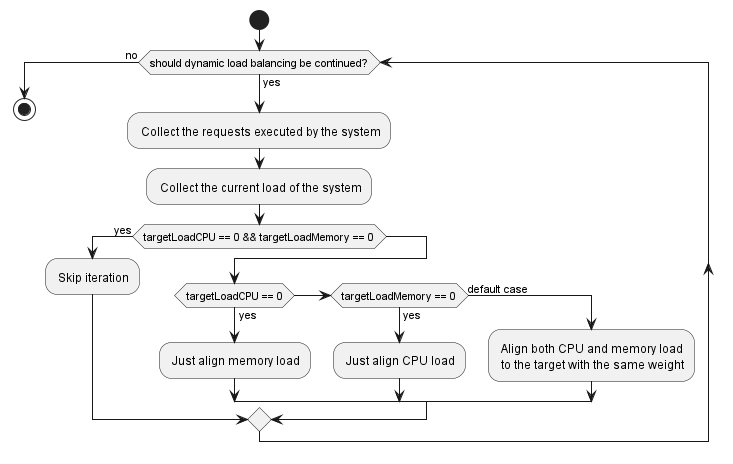
\includegraphics[width=\linewidth]{figures/profaastinate/load-balancer-schedule.png}
    \caption{These parameters allow adaptive fine-tuning of the Load Balancer's behavior to meet specific performance and resource utilization requirements. The following activity diagram illustrates the logic sequences within the Load Balancer, whereby the direct setting of maxParallelRequests leads to the termination of the while condition, so that the calculation is no longer dynamic.}
    \label{fig:og-profaastinate}
\end{figure}

%%% Beispiel ja oder nein? Folgendes von GPT
In order to better understand this, we assume a scenario with the parameters:
\begin{itemize}
    \item Number of executed function calls: 100
    \item Target load for CPU: 0.7
    \item Target load for memory: 0.6
    \item Used load for CPU: 0.8
    \item Used load for memory: 0.5
\end{itemize}

Using the provided formulas:
\[
\text{{desiredNumberMem}} = \dfrac{100 \times 0.6}{0.5} = 120
\]
\[
\text{{desiredNumberCPU}} = \dfrac{100 \times 0.7}{0.8} = 87.5
\]
\[
\text{{maxParallelRequests}} = \lceil \frac{120 + 87.5}{2} \rceil = \lceil 103.75 \rceil = 104
\]

In this example, the Load Balancer would be configured to allow a maximum of 104 parallel requests to maintain optimal performance considering both CPU and memory usage.

\subsubsection{Elastic Deployer}
\label{sec:elastic-deploy}
In general, the deployer is used to save resources in the deployment by automatically stopping function containers that have not been used for a certain time window, which is set to 1 minute by default. It saves all containers associated with Nuclio and how long they are still running.
To stop certain containers, it forwards stop requests to the dedicated deployer services for Docker or Kubernetes, which do this for it. The environment services are integrated through an abstract layer via an interface, so that new environments could easily be deployed using the same approach, which is consistent with our desire for a modular extensible architecture.
It also constantly communicates with the various schedulers to ensure that the required containers are running when they need to be called synchronously. It can also continue functions that have already been stopped via the interface.

It is important to note that while a Docker implementation was successfully implemented, the Kubernetes implementation could not be completed within the given timeframe as it became too complex. This component was an attempt to imitate the Premium feature of Nuclio. Various ideas were collected and implemented for this, but in the end, the components created was not sufficiently convincing in terms of performance, and the deployer was deactivated for the final evaluation. 

\subsubsection{Nexus}
\label{sec:nexus}
The Nexus, as its name suggests, serves as the central hub of our implementation. It is responsible for the connection between various components. Moreover, it initializes all other components, which include the schedulers and the necessary supportive components. Supportive components are components that provide data to schedulers, which are necessary for their strategy. One of those supportive components is the Load Balancer. The Nexus also manages the Nexus Queue and provides it to all components that need them. During its initialization, the Nexus starts the schedulers and supportive components. Additionally, it exposes a RESTful endpoint to dynamically start, stop, or configure schedulers and other supportive components during runtime. When the Nexus receives an asynchronous request, it extracts the deadline subsequently from it. Then, it transforms the request into a Nexus Queue entry, the entry consists of a function invocation and the extracted deadline, which is needed to index the entry.

\subsubsection{Nexus Queue}
\label{sec:nexus-queue}
The Nexus Queue integrates the delay logic, which is responsible for storing the function invocation entries until subsequent processing. We used the deadline to index the entries, meaning the first entire of the queue has the lowest deadline, and vice versa. Therefore we employed a Go Heap, which is a self-balanced tree structure and fits perfectly for the indexed entries. We opted for this approach over the initial implementation with PostgreSQL, due to its lightweight and sorted nature. In addition, it provides some performance benefits because the entries are stored within the memory. One drawback of this approach in contrast to the original implementation with PostgreSQL, is the missing data resilience. The entries are lost in case of a system failure.

We tried to keep the implementation of the Nexus Queue as straightforward as possible, due to its crucial role in being easily expansible in the future. Our design ensures and feasible integration of custom methods for specific use cases, allowing necessary enhancements to the queue. This flexibility enables the system to evolve.

\subsubsection{Base Scheduler}
\label{sec:base-scheduler}

In our implementation, we refactored the approach of a single scheduler to view it more as a group of independent components, rather than a single entity, enhancing their expandability. This approach aligns with the composite design pattern, popular in Go, allowing us to structure the schedulers as composite objects composed of smaller, individual components. Each scheduler shares a common core concept: extracting items from the Nexus queue based on specific conditions while considering external factors and then transforming these items into synchronous requests to Nuclio's dashboard for immediate execution. These schedulers operate at regular intervals, with the timeout duration between intervals adjustable alongside other custom parameters in the configuration.

When building custom schedulers, some conventions must be taken into consideration. The scheduler has to be initialized inside the Nexus and integrated within the list of known schedulers so that the Nexus can start it. The Nexus Queue must be passed to the scheduler during initialization. Furthermore, it needs methods to start, stop, and gather the status of the scheduler. A developer might use the existing schedulers as orientation. The Nexus will then use those methods to start and stop the scheduler upon initialization. The strategy of the scheduler is recommended to be implemented within its executeScheduler method. There are no limitations to that, but developers have to take care that the schedulers won't interfere with each other.


\subsection{Scheduler Types}
\label{sec:scheduler-types}
In the following section, we will provide detailed explanations of the various scheduler types implemented in our system. Our implementation proposes three different scheduler types, which are designed to target independent goals: The Deadline Scheduler, Idle Scheduler, and Bulk Scheduler.

Firstly, we will explain the Deadline Scheduler, which is responsible for meeting the deadlines of function invocations. Then, we will provide information for the Idle and Bulk schedulers, those schedulers are designed to minimize the impact on resources. Specifically, the Deadline Scheduler targets the reduction of cold starts. All of the implemented schedulers communicate with the Load Balancer.

To speed up development and improve the configurability of the system, we have also integrated support for starting and stopping all schedulers via the REST Api. Using the endpoints "/scheduler/{schedulername}/start" and "/scheduler/{schedulername}/stop", researchers can quickly start or stop the scheduler's operations as needed. This implementation speeds up the development process considerably and thus meets the non-functional requirement for configuration flexibility.

    \begin{figure}
        \centering
        \includegraphics[width=.9\linewidth]{figures/profaastinate/deadline_scheduler_example.pdf}
        \caption{An instance of the Deadline Scheduler. Assuming that the deadlines for $Entry_1$ and $Entry_2$ in the queue are below a specified threshold, the Deadline Scheduler removes these entries ($Entry_1$ and $Entry_2$) from the queue for processing. This involves executing synchronous function invocation requests for these entries.}
        \label{fig:deadline-scheduler-example}
    \end{figure}
    \subsubsection{Deadline Scheduler} 
\label{sec:deadline-scheduler}
The deadline scheduler ensures that every function invocation in the queue is processed before its deadline. This process is depicted in Figure \ref{fig:deadline-scheduler-example}. This is done by periodically checking the entry at the front of the queue, which is always the function invocation with the lowest deadline in the Nexus Queue. If the deadline of this task falls within a configured threshold, the scheduler executes the function invocation. This execution includes the removal of the entry from the queue and subsequent synchronous requests to Nuclio's Dashboard.

This process, of checking, removing, and finally sending a synchronous request, is done as long as the deadline of the first entry in the queue falls within the configured threshold. If there are no items left in the queue, meaning the deadline for the first items is later than the threshold, the scheduler pauses for a specified timeframe. In contrast to the other schedulers, it is not restricted by the Load Balancer. It can make as many parallel requests as needed to process every task falling within the deadline. However, the scheduler also registers its requests in the Load Balancer, meaning that it claims a slot in the Load Balancer for a parallel request before removal of the entry, and releases the slot after sending the request. It can allocate more slots than available, to fulfil its objective to process all entries before their deadline. This can lead to the potential blocking of other schedulers.



    \begin{figure}
        \centering
        \includegraphics[width=.9\linewidth]{figures/profaastinate/idle_scheduler_example.pdf}
        \caption{An instance of the Idle Scheduler. With a maximum parallel request constraint set to 3 by the Load Balancer, this scheduler operates independently of specific time frame deadlines for queued items. Instead, it systematically removes the first three entries from the queue and processes requests for each entry ($Entry_1$, $Entry_2$, and $Entry_3$), adhering to the maximum parallel request limit enforced by the Load Balancer.}
        \label{fig:idle-scheduler-example}
    \end{figure}
    \subsubsection{Idle Scheduler}
\label{sec:idle-scheduler}
The Idle Scheduler has a significant dependence on the Load Balancer because the Load Balancer constrains its functionality. It operates similarly to the Deadline Scheduler by running at periodic intervals. It also extracts the first entry from the queue. However, unlike the Deadline Scheduler, the deadline of the item does not need to fall within a configured deadline threshold. The Idle Scheduler can process as many concurrent tasks as allowed by the Load Balancer. The Idle Scheduler will only process new entries if there are free slots available. In contrast to the Deadline Scheduler, it cannot allocate more slots than the maximum parallel requests set by the Load Balancer. Additionally, it processes the first entries of the queue, meaning the invocations with the lowest deadline, similar to the Deadline Scheduler, due to the sorted nature of the queue. This process is illustrated in Figure \ref{fig:idle-scheduler-example}.


    \subsubsection{Bulk Scheduler} 
\label{sec:bulk-scheduler}

    \begin{figure}
        \centering
        \includegraphics[width=.9\linewidth]{figures/profaastinate/bulk_scheduler_example.pdf}
        \caption{An instance of the Bulk Scheduler. This scheduler operates by identifying the largest group of entries with the same function invocation, where the associated function worker is paused. It ensures that this group of entries does not surpass the maximum parallel request limit. Subsequently, the scheduler removes this group of entries and processes them accordingly ($Entry_1$, $Entry_3$, and $Entry_5$).}
        \label{fig:bulk-scheduler-example}
    \end{figure}

The third and final scheduler we implemented is the Bulk scheduler, which tries to reduce cold start times. These occur when a function worker is paused and started again for processing incoming function invocations. In the context of Kubernetes, this means that the replicas of the function workers are scaled to zero, consequently, no function workers are currently running for that function. Nuclio utilizes this idea by scaling unused function workers to zero. Nuclio only starts a function worker again if a function for the worker is invoked. Nuclio uses this concept to minimize the resource footprint of function workers which are not frequently requested.

However, a challenge arises using Nuclio because paused function workers might be periodically called in intervals where the function scales down before it's invoked again. Consequently, the container starts up every time the function is invoked. Those start-ups entail resource usage and increase the latency. The Bulk Scheduler is designed to address this issue. The concept behind this scheduler is to batch requests for paused containers. It aggregates function invocations for the same function and sends them in direct succession, thereby ensuring only one cold start for the initial function invocation. The subsequent invocations can use the already unpaused container. Therefore, the scheduler identifies the most entries in the Nexus Queue that invoke the same function, which is currently paused or scaled to zero, and invokes them, as depicted in Figure \ref{fig:bulk-scheduler-example}. This process is also done in periodic intervals. The Bulk Scheduler depends on the number of max parallel requests ensuring the system runs below its resource utilization target.

\section{Evaluation}\label{sec:evaluation}

% This section shows benchmark designs and results of each papers' implementation by us.
% sand and fusionize attempt to solve similar problems -> same evaluation and
% comparison: latency benchmark aimed at measuring network overheads
% profaastinate is different -> own evaluation:
% all evaluations' results are discussed together in section
% \ref{sec:discussion}

This section provides an overview of our benchmark designs and the results of
our implementation for each paper. SAND and \textsc{Fusionize} attempt to solve
similar problems, hence they share the same evaluation and are directly compared
to each other. We primarily focus on the latency benchmark designed to measure
network overheads. On the other hand, \textsc{ProFaaStinate} is different from
the other approaches and therefore requires its own specific evaluation. The
outcomes of all these evaluations will be collectively discussed in Section
\ref{sec:discussion}.

\subsection{Fusionize and SAND}

% for fusionize and sand we designed a benchmark aimed at isolating the network
% overhead to simulate cascading cold starts and double billing. We chose method
% best showcases end to end latencies between faas functions we decided for
% synthetic base load to investigate system's performance under maximum stress.

% To showcase maximum latency, we designed two tasks, shown in Figure X,
% \emph{interface} task and \emph{counter} task. The counter Task receives a
% number and returns the number, incremented by one. The interface task receives
% a \emph{destination} number by the user and invokes the counter task, starting
% with the number zero. The result of the counter task is then used to invoke
% the counter task again until the destination number is reached.

% This proposed load generator is unconventional, as it resides within the
% system under test. However, this design allows for function invocation within
% the platfrom and most importantly \emph{between} functions. To start the
% benchmark, only the interface task needs to be invoked with destination
% number and latency between invocation and result is to measured.

\subsubsection{Experiment Setup}
\label{subsubsec:evaluation:fusionize_and_sand:experiment_setup}

For \textsc{Fusionize} and SAND, we have constructed a benchmark with the
intention of isolating networking overhead. This is designed to simulate scenarios
involving cascading cold starts and double billing. We made this decision based
on our belief that this approach most effectively displays the end-to-end
latencies that can occur between FaaS functions. We chose to employ a synthetic
base load for our testing in order to examine the system's performance under
maximum stress.

In order to illustrate the maximum latency, we devised two tasks. These tasks,
which can be seen in Figure \ref{fig:bench}, are known as the \emph{interface}
and \emph{counter} tasks. The objective of the counter task is to receive a
number and return the same number after it has been increased by one. The
interface task works by accepting a \emph{destination} number supplied by the
user, then invoking the counter task, beginning with the number zero. Following
this, the result of the counter task is used to again invoke the counter task,
repeating until the destination number is reached.

Our proposed load generator has an unconventional design, as it resides within
the system under test (SUT). However, this design allows function invocation
within the platform, and, even more crucially, between functions. This is
important, as both Fusionize and SAND are revolving around the communication
between FaaS functions. To initiate the benchmark, only the interface task needs
to be invoked with the destination number. The latency between the invocation
and result must then be measured.

% - In a production setting, Nuclio is run in k8s cluster
% - We configured deployment of our approaches for k8s
% - For our benchmarks we deployed our system in local Minikube cluster

In a production environment, Nuclio operates within a k8s cluster. We have
successfully configured the deployment of our approaches for operation within
the k8s environments. For benchmarking purposes, we deployed our system within a
local Minikube\footnote{\url{https://minikube.sigs.k8s.io/}} cluster.

\begin{figure}
    \centering
    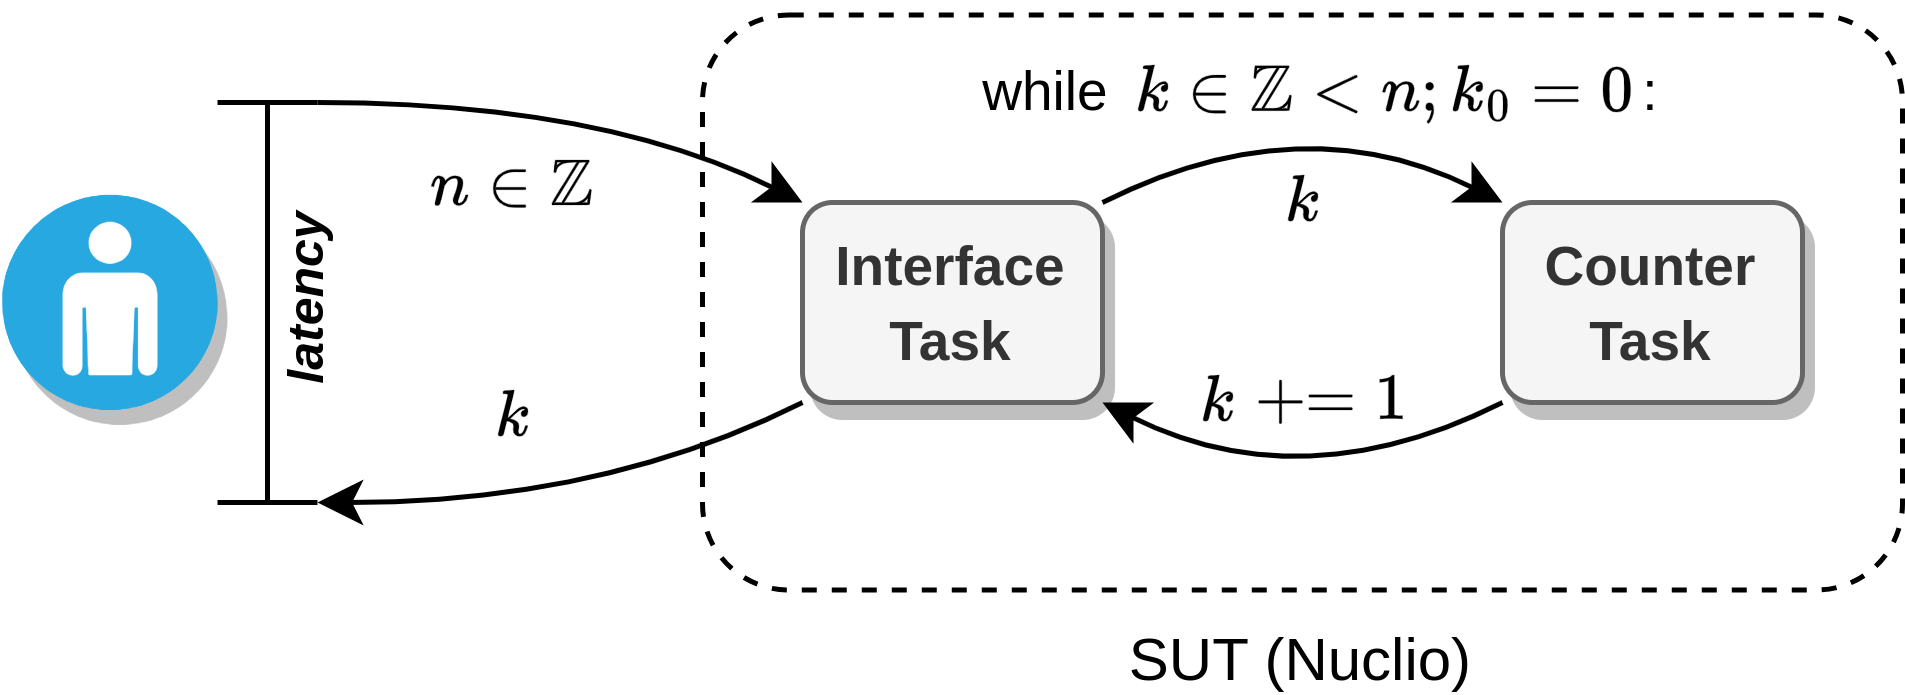
\includegraphics[width=\linewidth]{figures/bench}
    \caption{
        The Counter Task increments a given number by one. The Interface Task
        receives a target number from the user and repeatedly invokes the
        Counter Task, starting at zero, until the target number is achieved. The
        Interface Task then returns this number to the user upon completion of
        the benchmark run. This allows the user to measure the total end-to-end
        latency.
    }
    \label{fig:bench}
\end{figure}

\subsubsection{Results}
\label{subsubsec:evaluation:fusionize_and_sand:results}

\begin{figure}
    \centering
    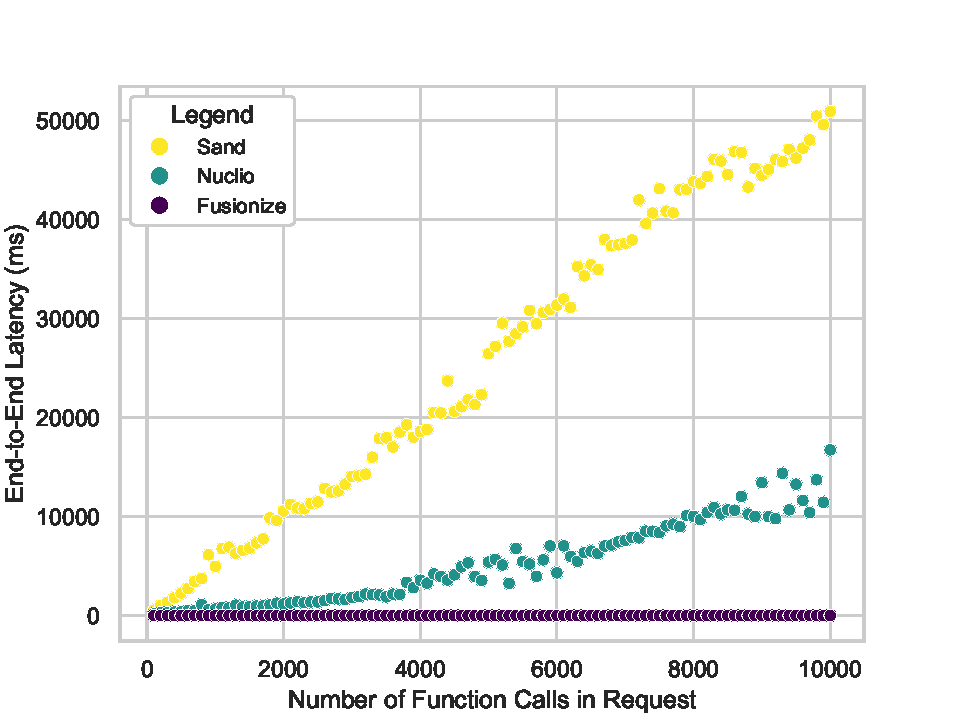
\includegraphics[width=\linewidth]{figures/latency_sand_fusionize}
    \caption{
        Results of our benchmark outlined in Figure \ref{fig:bench}. Our SAND
        implementation increases linearly and significantly faster than vanilla
        Nuclio. Our \textsc{Fusionize} implementation appears to have nearly
        constant latency.
    }
    \label{fig:latency_sand_fusionize}
\end{figure}


In Figure \ref{fig:latency_sand_fusionize}, we can see the results of our
benchmark. The x-axis shows the number of function calls required the answer the
request, and the y-axis show the measured end-to-end latency. As the interaction
between functions increases, the end-to-end latency increases linearly for SAND.
With 10,000 function calls, the SUT takes approximately 50 seconds to answer the
request using our SAND implementation. For vanilla Nuclio, the latency caused by
the same request if significantly lower at below 20 seconds. The end-to-end
latency of vanilla Nuclio scales exponentially with increasing interaction
between functions. With Fusionize, the latency is very close to 0 throughout the
experiment.


\subsection{ProFaaStinate}
\label{sec:eval-profaastinate}
In this section, we aim to evaluate the implementation status of both our functional and non-functional requirements as outlined in Section \ref{sec:functional-req}. To provide context for this assessment, we first outline our experiment setup, including the end-to-end test, and then present the results of the experiment. Finally, we analyze how well our system adheres to the defined requirements based on the results.

\subsubsection{Experiment Setup}

It is worth noting that we were unable to test the Bulk Scheduler in any meaningful way, as Nuclio only provides the scale to zero feature to enterprise users. We can confidently say that we did everything possible to implement that feature on our own, including a consultation with a developer from Nuclio. To the disadvantage of our experiment, we could not activate this feature. And without it, the integration of a Bulk Scheduler doesn't really make sense, although it does work.

In concrete terms, we aimed to evaluate the performance of ProFaaStinate when the Idle and Deadline schedulers are enabled. To achieve this, we devised a benchmark that subjects Nuclio to high load scenarios with asynchronous calls. By default, these calls are executed immediately in Nuclio, but with the schedulers enabled, they should be distributed evenly over time. The benchmark strategy involved imposing a constant load on Nuclio with a baseline of calls, while gradually increasing the load at intervals. We used k6, a load testing tool, to orchestrate and execute the benchmark.
The benchmark, which comprised function calls tasked with calculating prime numbers as well as executing functions named "vanilla" and "second", aimed at inducing high CPU utilization and compelling ProFaaStinate to delay certain calls. This setup initiated the benchmark with a base load of 800 requests having the deadline set to 4000 seconds. Subsequently, the benchmark sent a total of 800 requests at intervals, with the deadline between 5 seconds and 4000 seconds.
To ensure thorough validation of the implementation, we established an evaluation backend. This backend serves to record all function calls in the form of logs, enabling detailed analysis of the runtime information. The recorded data includes the following key attributes:
\begin{itemize}
    \item Function name: Identifies the specific function being called.
    \item Scheduler name: Specifies the scheduler responsible for managing the function's execution.
    \item Asynchronous  Deadline (timestamp)
    \item Start of synchronization processing (timestamp)
    \item Start of execution of function (timestamp)
    \item End of execution of function (timestamp)
\end{itemize}
We evaluated the benchmark within a Docker environment, as the performance of the Minikube environment proved to be inadequate—further details on this issue will be provided later. The tests were conducted on a system with the following specifications:
\begin{itemize}
    \item OS: Linux Mint 21.2 Cinnamon
    \item CPU: Inte i9-9900K
    \item RAM: 32GB
    \item GPU: AMD 6900xt
\end{itemize}

\subsection{Results}
% comparision
If required, our logs can be accessed directly via the Github repository to check our results\footnote{\url{https://github.com/valentin-carl/nuclio/tree/mpga-eval/profaastinate/evaluation/data-analysis/logs}}. 
We start with a comparison of how synchronous tasks in Nuclio without ProFaaStinate differ from asynchronous tasks with ProFaaStinate. 

\begin{figure}
    \centering
    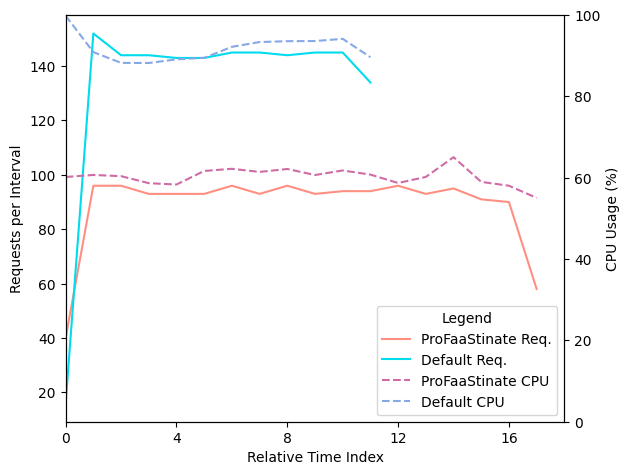
\includegraphics[width=\linewidth]{figures/profaastinate/results/line_chart.png}
    \caption{Default nuclio processing consumes higher peak CPU utilization and higher requests per interval, while ProFaaStinate processing requires a longer runtime.}
    \label{fig:metrics-comparision}
\end{figure}

In the graph \ref{fig:metrics-comparision}, the x-axis shows the relative time. This is a mapping of the timestamps of the default Nuclio and ProFaaStinate execution tests, which were executed one after the other and therefore had to be mapped to each other. The left y-axis describes the requests per interval, while the right y-axis shows the utilization of the system in relative time. There are 4 lines, with the red and orange ones referring to the ProFaaStinate calls and the bluish ones to the Default calls. 
It can be clearly seen that the Default lines are set higher than their respective counterparts. For example, the average CPU utilization in Default execution is around 90\%, while the utilization of the ProFaaStinate system is around 60\%. 
The situation is similar with the number of requests per interval in the standard setup, where around 140 are processed, while ProFaaStinate only processes 100. Default processing stops after about 10 time units, while ProFaaStinate processing continues until approximately 17. It should be noted that the level of CPU utilization in both modes is already relatively high at the beginning of the experiment and hardly decreases noticeably. It stands out that the standard processing is directly 100\% at the beginning.


\begin{figure}
    \centering
    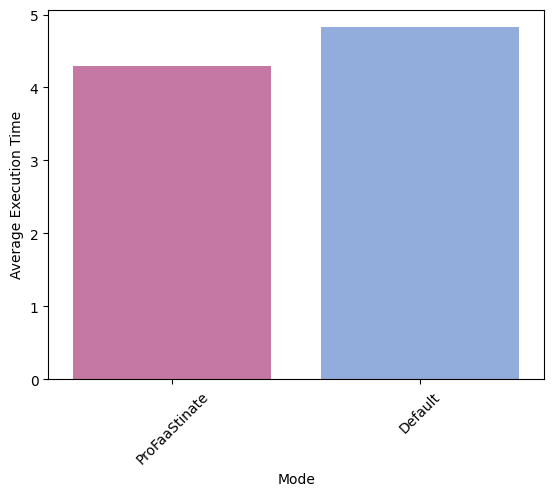
\includegraphics[width=\linewidth]{figures/profaastinate/results/execution_time_chart.png}
    \caption{ProFaaStinate Reduces Average Execution Time by 15\% Compared to Default Nuclio}
    \label{fig:execution-time-comparision}
\end{figure}

The diagram \ref{fig:execution-time-comparision} has the average execution time as the y-axis with values between 0 and 5. Meanwhile, the x-axis provides information about the mode, which is either ProFaaStinate or default Nuclio. While the average standard execution time is almost 5, with ProFaaStinate it is closer to 4.25. This means that function calls can be processed faster with ProFaaStinate than with default Nuclio.

\begin{figure}
    \centering
    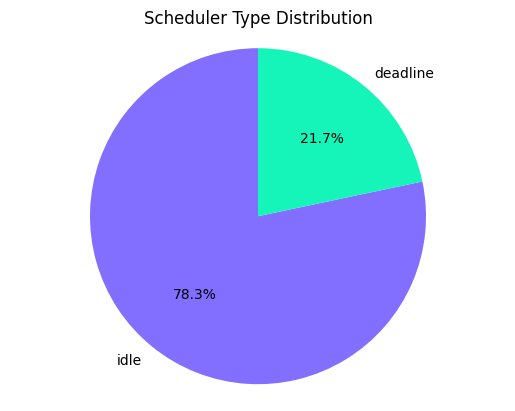
\includegraphics[width=\linewidth]{figures/profaastinate/results/pie_chart.png}
    \caption{
        Idle Scheduler Handles Majority of Function Invocations in ProFaaStinate
        %Results of the benchmark performed with ProFaaStinate implemented. It indicates the distribution between the Deadline Scheduler and the Idle Scheduler of processed entries. It shows that the Idle Scheduler processed the largest amount of function invocation requests.
    }
    \label{fig:scheduler-distribution}
\end{figure}
Having previously compared asynchronous and synchronous processing, we will now only focus on the insights of asynchronous processing.
Figure \ref{fig:scheduler-distribution} showcases the activity of the Idle and Deadline Scheduler during the benchmark with ProFaaStinate.  It indicates that the Idle Scheduler processed 78.3\% of the function invocation requests, and the Deadline Scheduler only processed 21.7\% of the function invocation requests. Consequently, the Idle Scheduler processed the largest number of requests.

\subsection*{Fullfillments of Functional Requirements}
The following section evaluates whether or not the functional requirements have been met. Relevant key figures from the test are used for this purpose. 
\begin{itemize}
    \item \textbf{Asynchronous function execution}: In our tests, all 1600 requests that were sent asynchronously to the Nuclio system triggered a callback on our evaluation backend. Since all requests arrived according to the protocols, every intermediate step, including the \nameref{sec:nexus-queue}, must function seamlessly. 
    Furthermore, we can observe in Figure \ref{fig:execution-time-comparision} that the execution time of requests, is slightly reduced, the reason for that is the CPU possible throtteling of the system, when operating at its processing limit. This effect could be particularly advantageous in environments in which synchronous and therefore time-critical requests also lie between the asynchronous requests. This is because, as explained in \nameref{sec:ProFaaStinate_Concept}, a calling component might wait for the response, hence latency plays a role. 
    This requirement is considered fulfilled.
    
    \item \textbf{Different Scheduler Types}: This requirement has been achieved by implementing the various scheduler types \nameref{sec:deadline-scheduler}, \nameref{sec:idle-scheduler} and \nameref{sec:bulk-scheduler}. Each scheduler type serves specific purposes and operates independently, ensuring that resources are optimally utilized and separation of concerns is respected. According to the logs and the benchmark (Figure \ref{fig:scheduler-distribution}), all tasks are executed within the deadline and both the idle and the Deadline Scheduler have processed function calls. We can therefore confirm that the simultaneous use of multiple schedulers is possible. However, the Deadline Scheduler only intervenes in an emergency to ensure timely processing.
    
    \item \textbf{Configuration Flexibility}: This requirement has also been met by offering both constructors as well as default factory constructors that enable smooth integration of components into the setup. In addition, we offer users the option of dynamically starting and stopping schedulers during runtime via a REST interface. The attributes of the Load Balancer can also be changed during runtime via REST, allowing the system to be fine-tuned to research requirements as required.
\end{itemize}

\subsection*{Fullfillments of Non-Functional Requirements}
After the functional requirements, the non-functional requirements must now be checked.
\begin{itemize}
    \item \textbf{Abstraction layer}: We have successfully implemented this requirement by integrating the entire logic of ProFaaStinate into our own package "Nexus". The Nexus package functions as a stand-alone unit and is only activated via a dashboard link and the deadline header. This ensures a clear separation between the integrated logic and the external components.
    \item \textbf{Modular extensible architecture}: In building our modular and extensible architecture, we applied key design patterns. We used the factory pattern to simplify component integration by providing default values where needed. Additionally, the composite pattern facilitated component structuring, particularly evident in models like the \nameref{sec:bulk-scheduler} and base scheduler. For complex deployment processes, we implemented the facade pattern with the \nameref{sec:elastic-deploy}, offering simplified interface for the schedulers to attach to instead of directly assigning the docker or kube environment. 
    In addition, the composite creation pattern was used to build new schedulers, see \nameref{sec:base-scheduler}. This system is based on the Load Balancer, which proves to be effective in its implementation. For the experiment, the described default values from the section \ref{sec:load-balancer} were used, where the Load Balancer should only allow new requests up to 60\% load. This does not work for a short time, as the load is closer to 70\% at time unit 14; this is corrected again directly in the next interval. This means that the scheduler creator does not have to worry about his scheduler overloading the system.
    This requirement is considered fulfilled.

    \item \textbf{Documentation}: In terms of documentation, our final submission included detailed README files covering all areas, as well as separate guides for deploying the software to Kubernetes and Docker environments. In addition, in-code documentation was provided for all Golang files to improve developers' understanding of the codebase. Futhermore, 9 UML diagrams have been created to illustrate workflow scenarios and component relationships within the system. With these documentation resources, users should be able to effectively understand the software and its architecture, fulfilling this requirement

    \item \textbf{Unit tests}
    Unfortunately, the targeted percentage of 75\% could not be achieved and in the end we only achieved a test coverage rate of 62.3\%. Factors that contributed to this shortfall include a lack of time, the complexity of the code base and a lack of experience in the project lanaguage Golang. However this deviation is probably still enough in a test project that primarily serves research purposes, but it remains the case that we were unable to fulfill this point.
\end{itemize}
\section{Discussion}\label{sec:discussion}

% 1) experiment: why 
% 2) nuclio doof
% 3) warum die 3 sub-projekte trotzdem gut sind

In this section, we first discuss the results of our experiments, offer possible explanation for the results we observed, and interpret them.
Next, we go over Nuclio to review how well Fusionize, SAND, and ProFaaStinate fit the platform, and we go over some drawbacks of using Nuclio we have experienced during the project. 
Lastly, we discuss the three subprojects in more detail.

\subsection{Interpretation of Experiment Results}

\subsubsection{Fusionize and SAND}

There are different possible explanations for the large differences between SAND, Fusionize, and vanilla Nuclio that we observed in our experiment.
To begin, all requests go through the Nuclio dashboard using vanilla Nuclio.
In this case, the dashboard creates a large performance bottleneck, as all function calls have to pass through it.
Going through the dashboard for every request adds a lot of steps for the execution of the workflow: To invoke the next step, the request leaves its current function pod, enters a different pod—containing the Nuclio dashboard—only to be routed to another function pod again.

In comparison, the request does not leave its pod during the workflow using SAND. 
With SAND, a function call goes from a function processor to the local message bus, to a grain worker, to another function processor.
In our experiment, we observed better scalability but (significantly) worse performance with regard to latency.
An explanation for this is the environment the experiment was conducted in.
It is possible that the end-to-end latency using SAND would be lower than the latency using SAND while deploying Nuclio on a larger Kubernetes cluster, which would give SAND's components more resources, allowing it to improve its performance.
However, further experiments are required to confirm or deny this.
Running on Minikube, the cost of invoking workflow steps is relatively high: Requests go from one function processor to another container—the local message bus—where RabbitMQ forwards the message to the next container, the grain worker, which—again—sends a request to the next container, where the function processor can execute the next function.

A difficulty for conducting experiments with Nuclio, in general, is its stability: Even with the load generated during our experiment, the platform crashed multiple times, requiring multiple experiment runs to obtain the results.
This problem occurred more frequently as the number of function calls required to answer a request increased.

Our Fusionize implementation maintains an apparently constant performance, which is attributable to tasks within the same fusion group residing in the same Nuclio function. 
These tasks are within the same process and therefore use the same memory space, which facilitates immediate execution. 
The benchmark for Fusionize is simply Python code executing a loop. 
Given this, latency is quite low and remains relatively constant for comparably low loads.

However, this does not necessarily mean our Fusionize implementation is the best option. 
There are potential scaling issues, particularly regarding the dependency on the configured optimization process. 
Fusion groups may be replicated, even if only one task experiences high load. 
If the optimization process is altered to accommodate this, all functions would need to be deleted, re-fused, and re-deployed, which could be time-intensive.

A possible solution to this would be the implementation of native \enquote{per task} scaling, instead of having Nuclio treat multiple functions as one entity. 
Unfortunately, this is not currently possible or feasible with Nuclio. 
It would require a significant rewrite of the core platform and its K8s interface, which is responsible for scaling.

\subsubsection{ProFaaStinate}

%• Experiments indicate the efficacy of ProFaaStinate:
%• Successfully demonstrates the ability to distribute load evenly over time.
 
The findings from our experiments provide insights into the performance of ProFaaStinate, shedding light on its potential implications for load management within serverless environments.
Through our evaluation, several key observations emerged: Firstly, ProFaaStinate demonstrates its capability to distribute workload evenly over time, which mitigates load spikes and ensures better resource utilization.

%• Proof of concept establishes its viability in reducing load spikes.
%• Implementation meets function invocation deadlines while mitigating load spikes.
%• Our implementation enhances the overall expandability compared to the initial implementation
%• Refactored the queuing mechanism to provide a more feasible approach of sorting and storing requests

Moreover, the proof of concept affirms ProFaaStinate's ability to reduce load spikes by strategically delaying workload execution.
Furthermore, our implementation of ProFaaStinate meets function invocation deadlines and efficiently mitigates load spikes, which is crucial for maintaining system stability and performance.
An important aspect of our implementation is the improved expandability compared to the initial version.
By refactoring the queuing mechanism, we've devised a more feasible approach for sorting and storing requests, laying a robust foundation for future scalability.

%• Evaluation challenges due to Nuclio limitations:
%    - Nuclio dashboard presents significant bottleneck.
%    - Local usage with Minikube yields throughput below 1 request per function worker.
%    - Docker deployment marginally improves throughput; hence, evaluation conducted with Docker.
%    - Enterprise features such as scale-to-zero mode in Nuclio, essential for Bulk scheduler, are unavailable for standalone implementation.
%        * Implementing such features within Nuclio independently is complex.

However, it's essential to acknowledge the challenges encountered during evaluation, primarily stemming from limitations within the Nuclio platform.
The Nuclio dashboard emerged as a bottleneck, hindering efficient monitoring and management of functions.
Running Nuclio locally via Minikube yielded a throughput of below one request per function worker per second.
Conversely, deploying Nuclio on Docker marginally improved throughput, albeit with some complexities, which is why we conducted the evaluation of ProFaaStinate on Docker.
Furthermore, the absence of enterprise features, particularly the scale-to-zero mode in Nuclio that was essential for the bulk scheduler, poses limitations and complicated independent implementation within Nuclio.

%• Despite being a proof of concept, ProFaaStinate demonstrates potential benefits:
%    - Offers promise in reducing load spikes by evenly delaying workload to specified time frames.
%    - Establishes a foundation for implementing other schedulers, adhering to common conventions for convenient implementation.
%    - Provides an opportunity to enhance previous implementations of ProFaaStinate for improved performance and functionality

Despite these challenges, ProFaaStinate shows potential benefits in reducing load spikes and establishing a foundation for implementing other schedulers in serverless environments.
While ProFaaStinate remains a proof of concept, our experiments provide a foundation for insights into its performance and potential implications for load management in serverless environments.
Further exploration and optimization are required to fully understand its capabilities and refine its functionality in practical applications.

\subsection{Nuclio}

%- Nuclio proved to be challenging in different regards during the project
%- Deployments
%    - Kubernetes Documentation was a main challenge and larger part of the project than anticipated
%    - However, we made it!
%    - In addition, even after figuring out how Nuclio works with Kubernetes ourselves, it is still not frictionless
%        => for example, build times are enormous at, in some cases, > 1 hour
%        => also, the hardware requirements for deploying Nuclio onto GKE are even larger (which made it unusable for large parts of the project)
%- Fusionize
%    - native implementation requires re-writes of large parts of the Nuclio codebase 
%    - -> infeasible 
%    - -> just do from scratch or use other FaaS platform
%- SAND
%    - Nuclio's design decision—the use of Kubernetes as backend—dictates our design decisions for implementing application sandboxing with pods
%    - Given the general alternatives for application sandboxing, Kubernetes pods are a very large unit, which comes at the cost of performance
%    - Because of our use of pods, the networking overhead for SAND is still quite high (as seen in the experiments)
%    - For the design of a serverless platform, the level of isolation between functions is important, comes early, and influences the rest of the platform's design significantly
%        - For Nuclio, a decision was made to separate individual function as much as possible => different pods for each function allows scaling, monitoring, restarting, ... them individually
%        - In contrast, SAND is a complete serverless platform built for the purpose of application sandboxing
%        - Naturally, it is going to perform far better than a platform that was not built with sandboxing in mind and that was only retrofitted with that capability
%- ProFaaStinate
%    - The ProFaaStinate ran into challenges related to Nuclio's enterprise features, which are not supported/documented in the open-source variant
%    - In addition, the dashboard (as in the platform's gateway) limits its performance -> a different load balancer would be required to benchmark the impact of ProFaaStinate more toroughly
%- Performance
%    - Dashboard
%        - Nuclio was built to expose functions directly (-> function ingress), hence the dashboard is not intended to be use as a high performance load balancer (which we would like!)
%    - Kubernetes overhead
%        - In general, the overhead of Kubernetes is quite high => particularly for the use as the backend of a FaaS platform
%        - ...

In the course of our project, Nuclio present us with multiple noteworthy challenges over the course of our project.

To begin, deployments proved to be more complex than anticipated, with navigating the Kubernetes documentation—or lack there of—consuming a larger portion of our project timeline than initially expected.
Despite these obstacles, we ultimately succeeded in deploying our system with the Kubernetes backend, in addition to Docker. 
However, even after gaining a deeper understanding of Nuclio's integration with Kubernetes, the deployment process remained less than frictionless.
Prolonged build times, sometimes exceeding an hour, posed a significant challenge.
Furthermore, the hardware requirements for deploying Nuclio onto Google Kubernetes Engine (GKE) proved to be prohibitively large for certain components of our project.

Attempting a native implementation of Fusionize within Nuclio presented formidable challenges.
Extensive rewrites of the Nuclio codebase would have been necessary, rendering this approach infeasible, which dictated the design of our implementation.

The architectural decision of Nuclio to use Kubernetes as its backend significantly influenced our approach to implementing application sandboxing with pods.
However, using Kubernetes pods as the unit of isolation for SAND introduced significant performance overhead, particularly in terms of networking.
This underscores the importance of early design decisions in the development of a serverless platform, as the level of isolation between functions significantly impacts overall performance and independent scalability of functions.
While SAND does not use Kubernetes pods for isolation, it's essential to note that SAND is purpose-built for application sandboxing, which gives it a natural advantage over platforms retrofitted with sandboxing capabilities like Nuclio.

ProFaaStinate faced hurdles related to Nuclio's enterprise features, which are either unsupported or poorly documented in the open-source variant.
Moreover, limitations within the platform's dashboard constrained performance significantly. 
One possibility of realize the full potential of ProFaaStinate is the exploration of alternative load balancers for more comprehensive benchmarking.

Regarding performance, Nuclio's architecture, designed to expose functions directly, implies that its dashboard is not optimized for high-performance load balancing, posing challenges for systems that rely on it like ours.
Additionally, the inherent overhead of Kubernetes, particularly when used as the backend for a FaaS platform, can significantly impact performance.

%Our experience with Nuclio shed light on various technical and operational challenges, emphasizing the complexities involved in deploying and managing serverless platforms.
%These insights provide valuable considerations for future research and development efforts in the field of cloud computing and serverless architectures.

\subsection{Fusionize, SAND, and ProFaaStinate}

%- While Nuclio might not have been a perfect fit for the three (which was to be expected with Nuclio not being built with these in mind), they are still very useful additions 
%- Fusionize performed better than SAND is it takes the idea of \enquote{two-level fault isolation} to its logical conclusion
%- While it would constitute a major design change, replacing Nuclio's individual function pods with native sandboxes could lead to significant performance benefits
%- The relevance of managing load spikes by spreading requests out over time can be seen by real-world implementations such as XFaaS, which made use of the approach after it had been introduced in ProFaaStinate 
%- As seen in our implementation, the Fusionize and SAND can each be combined with ProFaaStinate, which naturally fits for scheduling FaaS workflows
%- Function fusion and scheduling as in ProFaaStinate both lead to more efficient resource use, which is of universal interest
%    - platform owner can increase their profits if the hardware they use is better utilized
%    - application developers can make performance gains by taking shortcuts in communication between functions
%    - the same applies to the use of self-hosted FaaS-platforms, which benefits from both increased performance and more efficient resource use, too
%- Despite the drawbacks of Nuclio, the benefits of the three approaches became very clear
%- However, they would become even more clear in a FaaS platform that was designed with them in mind from the beginning

While Nuclio may not have been specifically tailored for the three approaches we explored, they nonetheless offer valuable contributions to the platform.

First, we observed that Fusionize greatly outperformed SAND by taking the concept of \enquote{two-level fault isolation} to its logical conclusion of reducing isolation between functions of the same application as far as possible.
Nonetheless, while it would constitute a major design change, replacing Nuclio's individual function pods with native sandboxes could lead to significant performance benefits

Next, the importance of managing load spikes by distributing requests over time is underscored by real-world implementations such as XFaaS~\cite{xfaas}, which adopted this approach following its introduction in ProFaaStinate.
In addition, our implementation demonstrated that Fusionize and SAND can seamlessly integrate with ProFaaStinate~\cite{schirmer2023profaastinate}, aligning naturally with scheduling FaaS workflows.

Both function fusion and scheduling, as demonstrated in Fusionize, SAND, and ProFaaStinate, contribute to more efficient resource utilization—a concept of universal interest.
Platform owners stand to increase profits through better hardware utilization, while application developers can achieve performance gains by optimizing communication between functions.
Similarly, self-hosted FaaS platforms benefit from enhanced performance and resource efficiency.

Despite the challenges posed by Nuclio, the benefits of the three approaches became evident.
However, their full potential would be even more pronounced in a FaaS platform designed with them in mind from inception.

In summary, while Nuclio may not have been initially engineered for these approaches, their implementation underscores their relevance and potential benefits in the realm of serverless computing.
These insights emphasize the value of incorporating such considerations into the design of future FaaS platforms to maximize efficiency and performance.

\section{Conclusion}\label{sec:conclusion}

Challenges associated with Function-as-a-Service (FaaS) platforms, such as high
costs due to double billing, latency issues from cascading cold starts, and
inefficiencies in synchronous and asynchronous function calls, have been
addressed through novel approaches like \textsc{Fusionize}, SAND, and
\textsc{ProFaaStinate}. Our Project explored the integration of these approaches
within the open-source serverless platform Nuclio.

Our findings indicate that these approaches have the potential to enhance the
overall efficiency and resource utilization within serverless computing
platforms. However, Nuclio posed as an impractical choice of a FaaS platform due
to its instability, design decisions, and performance overheads. In general, the
potential of these approaches is limited by container orchestration systems that
are not designed for FaaS applications, like Kubernetes. We believe that these
solutions will yield better results if they are integrated on a platform
specifically engineered for them.


%\balance

\bibliographystyle{IEEEtran}
\bibliography{bibliography}

\section*{Author Attribution}

% Usage: Name & \ref{sec:section} \\

\vspace{1em}
\begin{center}
    \begin{tabular}{l l} \toprule
        Name & Sections \\ \midrule
        Valentin Carl & \ref{sec:sand}, \ref{sec:evaluation}, \ref{sec:discussion} \\
        Daniel Gottschling & \ref{sec:sand}, \ref{sec:evaluation} \\
        Jonas Heisterberg & \\
        David Schmidt & \\
        Marvin Steinke & \ref{sec:introduction}, \ref{sec:fusionize}, \ref{sec:evaluation} \\ \bottomrule
    \end{tabular}
\end{center}

\end{document}
